\documentclass[oneside,letterpaper,titlepage]{article}
%\usepackage[ae,hyper]{/usr/lib/R/share/texmf/Rd}
\usepackage{graphicx}
\usepackage{natbib}
\usepackage[reqno]{amsmath}
\usepackage{amssymb}
\usepackage{verbatim}
\usepackage{epsf}
\usepackage{url}
\usepackage{html}
\usepackage{dcolumn}
\usepackage{fullpage}
\newcolumntype{.}{D{.}{.}{-1}}
\newcolumntype{d}[1]{D{.}{.}{#1}}
%\pagestyle{myheadings}
\htmladdtonavigation{
  \htmladdnormallink{%
    \htmladdimg{http://gking.harvard.edu/pics/home.gif}}
  {http://gking.harvard.edu/}}
\newcommand{\hlink}{\htmladdnormallink}

\bodytext{ BACKGROUND="http://gking.harvard.edu/pics/temple.jpg"}
\setcounter{tocdepth}{2}

\newcommand{\MatchIt}{\textsc{MatchIt}}

\title{\MatchIt: Nonparametric Preprocessing for Parametric Causal
  Inference}

\author{Daniel E. Ho,\thanks{J.D.\ candidate, Yale Law School, Ph.D.\,
    Department of Government, Harvard University. (Center for Basic
    Research in the Social Sciences, 34 Kirkland, Cambridge MA 02138,
    USA; \texttt{daniel.ho@Yale.Edu}).}
\and
Kosuke Imai,\thanks{Assistant Professor, Department of Politics,
  Princeton University (Corwin Hall 041, Department of Politics,
  Princeton University, Princeton NJ 08544, USA;
  \texttt{http://www.princeton.edu/\~{}kimai},
  \texttt{kimai@Princeton.Edu}).}
\and
Gary King,\thanks{David Florence Professor of Government, Harvard
  University (Institute for Quantitative Social Science, 34
  Kirkland Street, Harvard University, Cambridge MA 02138;
  \texttt{http://GKing.Harvard.Edu}, \texttt{King@Harvard.Edu}, (617)
  495-2027).}
\and
Elizabeth A. Stuart\thanks{Researcher, Mathematica Policy Research,
  Inc.\, Ph.D.\, Department of Statistics, Harvard University. (600
  Maryland Ave., SW, Suite 550, Washington, DC 20024, USA;
  \texttt{http://www.mathematica-mpr.com},
  \texttt{EStuart@Mathematica-MPR.com}).}}

\makeindex

\begin{document}
\maketitle

\begin{rawhtml}
  <p> [Also available is a downloadable <a
  href="/matchit/docs/matchit.pdf">PDF</a> version of this entire
  document]
\end{rawhtml}

\tableofcontents

%%%%%%%%%%%%%%%%%%%%%%%%%%%%%%%%%%%%%%%%%%%%%%%%%%%%%%%%%%%%%%%%%%%%%%%%
\clearpage
\section{Introduction}
\MatchIt\ implements the suggestions of \citet{HoImaKin05} for
improving parametric statistical models and reducing model dependence
by preprocessing data with semi- and non-parametric matching methods.
After preprocessing with \MatchIt, researchers can use whatever
parametric model they would have used without \MatchIt, but produce
inferences that are substantially more robust and less sensitive to
modeling assumptions.  Matched data sets created by \MatchIt\ can also
be entered easily into \hlink{Zelig}{http://gking.harvard.edu/zelig/}
\citep{ImaKinLau04}, or other programs, for subsequent parametric
analyses.  \MatchIt\ reduces the dependence of causal inferences on
commonly made, but hard-to-justify, statistical modeling assumptions
via a wide range of sophisticated matching methods.  In addition, we
have written \MatchIt\ so that adding methods to its structure is
easy, if you have the inclination.

\subsection{Software Requirements} 
\MatchIt\ works in conjunction with the R programming language and
statistical software, and will run on any platform where R is
installed (Windows, Unix, or Mac OS X).  R is available free for
download at the Comprehensive R Archive Network (CRAN) at
\hlink{http://www.r-project.org/}{http://www.r-project.org/}.
\MatchIt\ has been tested on the most recent version of R.  A good way
to learn R, if you don't know it already, is to learn Zelig (available
at \hlink{http://gking.harvard.edu}{http://gking.harvard.edu}) which
includes a self-contained introduction to R and can then be used to
analyze the data after \MatchIt.

\subsection{Installing \MatchIt}

To install \MatchIt\ for all platforms, type at the R command prompt:
\begin{verbatim}
install.packages("MatchIt")
\end{verbatim}
and \MatchIt\ will install itself onto your system automatically.
During the process you may either decide to keep or discard the
installation files, which will not affect the way \MatchIt\ runs.  You
only need to do this once.

\subsection{Loading \MatchIt}
As with any R package, you must install \MatchIt\ only once, but you
must load it prior to each use.  You can do this for each R session by
typing:
\begin{verbatim}
library(MatchIt) 
\end{verbatim}
at the R command prompt.  Alternatively, you can specify R to load
\MatchIt\ automatically at launch so that you can skip the step of
typing {\tt library(MatchIt)} at the beginning of every R session.  To
do this, edit the {\tt Rprofile} file located in the R program
subdirectory, e.g. \texttt{C:/R/rw1091/etc/}, for Windows systems or
the {\tt .Rprofile} file located in the home directory for Unix/Linux
and Mac OS X systems.  Using a text editor such as Windows notepad and
emacs, add the following line to the file:
\begin{verbatim}
options(defaultPackages = c(getOption("defaultPackages"), "MatchIt"))
\end{verbatim}
For this change to take effect, you need to restart R.

%%%%%%%%%%%%%%%%%%%%%%%%%%%%%%%%%%%%%%%% shall we add this back in?
% \subsection{Updating \MatchIt}
% You may update to the most recent version of \MatchIt\ by typing the
% following commands from your R session.
%
% \begin{small}
% \begin{verbatim}
%> update.packages("MatchIt")
%> library(MatchIt) 
%\end{verbatim}
% \end{small}

%%%%%%%%%%%%%%%%%%%%%%%%%%%%%%%%%%%%%%%%%%%%%%%%%%%%%%%%%%%%%%%%%%%%%%%%


\section{Statistical Overview}
\label{sec:overview}

{\bf Here, we describe the idea of using matching as preprocessing.
  Maybe, the example should be in A User's Guide?}

Once the matching is complete, the \MatchIt\ object can be used with
any other analysis procedure; \MatchIt\ is designed to make those
analysis procedures less dependent on the modeling assumptions and
thus work better.  Therefore, any analysis you might have done using
the original data sets can be done better on the matched data sets.
To obtain the matched data sets, use {\tt match.data(m.out)}, where
{\tt m.out} is a \MatchIt\ object. See Section~\ref{subsec:match.data}
for more options and details.

In this section, we describe our recommended approach
\citep{HoImaKin05}, which uses
\hlink{Zelig}{http://gking.harvard.edu/zelig/} to conduct parametric
causal inference after preprocessing the data through \MatchIt.  The
resulting matched data sets can also be exported to other statistical
program using commands such as {\tt write.table()} and {\tt
  write.csv()}. Also, the commands in the {\tt foreign} package allow
users to save matched data sets as binary files for various
statistical software including STATA and SPSS.

Zelig \citep{ImaKinLau04} is an easy-to-use R package that estimates a
variety of statistical models, gives easily interpretable results by
simulating quantities of interest, and provides numerical and
graphical summaries.  The package along with the complete
documentation is available at
\hlink{http://gking.harvard.edu/zelig/}{http://gking.harvard.edu/zelig/}.
\MatchIt\ and Zelig can be easily used together to enable estimation
of causal effects in very general settings with a variety of
statistical models.

The general framework is that of imputing the missing potential
outcomes.  For example, for the treated group, the potential outcomes
under control, $Y_{0i}$, are missing, whereas the outcomes under
treatment, $Y_{1i}$, are observed.  We impute the missing outcomes,
$Y_{0i}$, via Monte Carlo simulation using a parametric statistical
model as follows.  First, we fit a model using the observed outcomes
of the matched control units (i.e., using only observations where
$T_i=0$).  Then, given this fitted model, the missing outcomes
$Y_{i0}$ are imputed for the matched treated units by using the values
of the explanatory variables for the treated units.  Once those
potential outcomes are imputed, the estimate of individual $i$'s
treatment effect is $Y_{1i}-\widehat{Y}_{0i}$ where $\widehat{Y}_{0i}$
is the Monte Carlo estimate of the average missing potential outcome
for unit $i$.  The in-sample average treatment effect for the treated
individuals can be then obtained by averaging over $i$ of this
difference. A similar procedure can also be used to estimate various
quantities of interest. Another advantage of this simulation approach
is that the uncertainty estimates such as standard errors are obtained
easily from the estimation uncertainty in fitting the parametric
model. See \citep{HoImaKin05} for more details.



For any matching procedure, \MatchIt\ does its work with the following
three commands:

\begin{enumerate}
\item \texttt{matchit()} implements a variety of matching procedures.

\item \texttt{summary()} summarizes the resulting balance of
  covariates after matching.

\item \texttt{plot()} creates plots useful for balance diagnostics.
\end{enumerate}

In addition, \texttt{match.data()} creates the data frame from the
original data frame by excluding unmatched units and including
information about the particular matching procedure (i.e., weights,
subclasses, and distance measure).  This matched data set can then be
used for subsequent parametric analyses thorough
\hlink{Zelig}{http://gking.harvard.edu/zelig/} or other statistical
programs. Finally, a standard \texttt{print()} command can be used to
print out a very brief summary of the output object.

In this section, we describe our recommended approach
\citep{HoImaKin05}, which uses
\hlink{Zelig}{http://gking.harvard.edu/zelig/} to conduct parametric
causal inference after preprocessing the data through \MatchIt.  (The
resulting matched data sets can also be exported to other statistical
programs using commands such as {\tt write.csv()} and {\tt
  write.table()} for ASCII files, and {\tt write.dta} in {\tt foreign}
package for a STATA binary file.)  Zelig \citep{ImaKinLau04} is an
easy-to-use R package that implements a large variety of statistical
models, gives easily interpretable results by simulating quantities of
interest, provides numerical and graphical summaries, and is easily
extensible.  The package along with the complete documentation is
available at
\hlink{http://gking.harvard.edu/zelig/}{http://gking.harvard.edu/zelig/}.
\MatchIt\ and Zelig can be easily used together to enable estimation
of causal effects in very general settings with a variety of
statistical models.

The general syntax is as follows. First, we use \texttt{match.data()}
to create the matched data by excluding unmatched units from the
original data, and including information about the particular matching
procedure (i.e., weights, subclasses, and the distance measure).
\begin{Schunk}
\begin{Sinput}
> m.data <- match.data(m.out)
\end{Sinput}
\end{Schunk}
where {\tt m.out} is the \MatchIt\ object from {\tt matchit()} and
{\tt m.data} is the resulting matched data.  Next, we analyze the
matched data set via the following command,
\begin{Schunk}
\begin{Sinput}
> z.out <- zelig(Y ~ treat + x1 + x2, model = mymodel, data = m.data)
\end{Sinput}
\end{Schunk}
where {\tt Y} is the outcome variable, {\tt mymodel} is the selected
model, and {\tt z.out} is the output object from {\tt zelig}.

To illustrate this approach, we provide two detailed examples using
the Lalonde data. Users can run these example commands by typing {\tt
  demo(Zelig)} at the R prompt. Although we use the linear least
squares model in these examples, a wide range of other models are
available in Zelig (for the list of supported models, see
\hlink{http://gking.harvard.edu/zelig/docs/Models\_Zelig\_Can.html}{http://gking.harvard.edu/zelig/docs/Models_Zelig_Can.html}).
If you have not installed Zelig, follow the installation procedure
described at
\hlink{http://gking.harvard.edu/zelig/docs/Installation.html}{http://gking.harvard.edu/zelig/docs/Installation.html}
To load the Zelig package after installing it, type

\begin{Schunk}
\begin{Sinput}
> library(Zelig)
\end{Sinput}
\end{Schunk}

\paragraph{Examples}
\begin{enumerate}
\item We begin our first example by conducting the nearest neighbor
  matching using the estimated propensity score from the logistic
  regression
\begin{Schunk}
\begin{Sinput}
> m.out1 <- matchit(treat ~ age + educ + black + hispan + 
+     nodegree + married + re74 + re75, method = "nearest", 
+     data = lalonde)
\end{Sinput}
\end{Schunk}
Note that we skip an important step of checking balance in this
example in order to focus on the illustration of analyzing matched
data sets. We then fit the linear model to the control group
controlling for the estimated propensity score and other covariates,
\begin{Schunk}
\begin{Sinput}
> z.out1 <- zelig(re78 ~ age + educ + black + hispan + nodegree + 
+     married + re74 + re75 + distance, data = match.data(m.out1, 
+     "control"), model = "ls")
\end{Sinput}
\end{Schunk}
where the {\tt "control"} option in {\tt match.data()} extracts the
matched control units and {\tt ls} specifies linear regression. Note
that we need not include the treatment indicator in this regression.
Next, we set the covariates to the covariate values of the matched treated units
and use conditional prediction by setting the {\tt setx()} command optionsn to {\tt cond = TRUE} and {\tt
  fn = NULL} in order to impute the
counterfactual outcomes for the treated units. The {\tt sim()} command in
Zelig does the imputation.
\begin{Schunk}
\begin{Sinput}
> x.out1 <- setx(z.out1, data = match.data(m.out1, "treat"), 
+     fn = NULL, cond = TRUE)
> s.out1 <- sim(z.out1, x = x.out1)
\end{Sinput}
\end{Schunk}
Finally, we obtain a summary of the results by 
\begin{Schunk}
\begin{Sinput}
> summary(s.out1)
\end{Sinput}
\begin{Soutput}

  Model: ls 
  Number of simulations: 1000 

Mean Values of Observed Data (n = 185) 
(Intercept)         age        educ       black      hispan    nodegree 
  1.000e+00   2.582e+01   1.035e+01   8.432e-01   5.946e-02   7.081e-01 
    married        re74        re75    distance 
  1.892e-01   2.096e+03   1.532e+03   5.774e-01 

Pooled Expected Values: E(Y|X)
   mean      sd    2.5%   97.5% 
 4989.5  2304.9   684.1 10027.6 

Pooled Average Treatment Effect: Y - EV
  mean     sd   2.5%  97.5% 
1359.6  593.3  248.4 2590.4 

\end{Soutput}
\end{Schunk}
The results indicate that the estimated average treatment effect on
the treated is 
\$1359.6,
with a 95\% interval of
(\$248.4,
\$2590.4).

It is also possible to estimate the average treatment effects on both
the treated and the control groups. To do this, we fit the linear
model to the {\it treatment group} controlling for the propensity
score ({\tt distance}) and other covariates,
\begin{Schunk}
\begin{Sinput}
> z.out2 <- zelig(re78 ~ age + educ + black + hispan + nodegree + 
+     married + re74 + re75 + distance, data = match.data(m.out1, 
+     "treat"), model = "ls")
\end{Sinput}
\end{Schunk}
We then conduct the same simulation procedure in order to impute the
counterfactual outcome for the {\it control group},
\begin{Schunk}
\begin{Sinput}
> x.out2 <- setx(z.out2, data = match.data(m.out1, "control"), 
+     fn = NULL, cond = TRUE)
> s.out2 <- sim(z.out2, x = x.out2)
\end{Sinput}
\end{Schunk}
Finally, note that Zelig calculates the difference between observed
and either predicted or expected values.  This means that the
treatment effect for the control units is actually the effect of
control (observed control outcome minus the imputed outcome under
treatment from the model).  Hence, to combine treatment effects just
reverse the signs of the estimated treatment effect of controls.
\begin{Schunk}
\begin{Sinput}
> ate.all <- c(s.out1$qi$ate.ev, -s.out2$qi$ate.ev)
\end{Sinput}
\end{Schunk}
The point estimate and its standard error is given by
\begin{Schunk}
\begin{Sinput}
> mean(ate.all)
\end{Sinput}
\begin{Soutput}
[1] 1624

\end{Soutput}
\begin{Sinput}
> sd(ate.all)
\end{Sinput}
\begin{Soutput}
[1] 794.5

\end{Soutput}
\end{Schunk}
The 95\% confidence interval is given by
\begin{Schunk}
\begin{Sinput}
> quantile(ate.all, c(0.025, 0.975))
\end{Sinput}
\begin{Soutput}
  2.5%  97.5% 
 205.3 3320.5 

\end{Soutput}
\end{Schunk}
  
\item Our second example is subclassification. In this case, the
  average treatment effect estimates are obtained separately for each subclass
  as well as for the overall sample.  Estimating the
  treatment effects separately for each subclass, and then aggregating
  across subclasses, can significantly increase the robustness of the
  ultimate results since the parametric analysis within each subclass
  requires only local rather than global assumptions.

  We begin this example by conducting subclassification with four subclasses,
\begin{Schunk}
\begin{Sinput}
> m.out2 <- matchit(treat ~ age + educ + black + hispan + 
+     nodegree + married + re74 + re75, data = lalonde, method = "subclass", 
+     subclass = 4)
\end{Sinput}
\end{Schunk}
Here, we skip the important step of checking balance in order to focus
on the illustration of analyzing subclassified data sets.  Next, we
fit the linear regression within each subclass by controlling for the
estimated propensity score and past income variables within each
subclass by using the {\tt by} option in the {\tt zelig()} command. 
\begin{Schunk}
\begin{Sinput}
> z.out3 <- zelig(re78 ~ re74 + re75 + distance, data = match.data(m.out2, 
+     "control"), model = "ls", by = "subclass")
\end{Sinput}
\end{Schunk}
The same set of commands as in the first example are used to
do the imputation of the counterfactual outcomes for the treated
units.
\begin{Schunk}
\begin{Sinput}
> x.out3 <- setx(z.out3, data = match.data(m.out2, "treat"), 
+     fn = NULL, cond = TRUE)
> s.out3 <- sim(z.out3, x = x.out3)
\end{Sinput}
\end{Schunk}
Finally, to obtain the overall results, type
\begin{Schunk}
\begin{Sinput}
> summary(s.out3)
\end{Sinput}
\begin{Soutput}

  Model: ls 
  Number of simulations: 250 

Mean Values of Observed Data (n = 46) 
(Intercept)        re74        re75    distance 
     1.0000   5430.5389   2929.0394      0.2392 

Pooled Expected Values: E(Y|X)
 mean    sd  2.5% 97.5% 
 4453  5150 -4994 15742 

Pooled Average Treatment Effect: Y - EV
  mean     sd   2.5%  97.5% 
1898.2 1691.6 -793.5 5478.9 

\end{Soutput}
\end{Schunk}
The results indicate that the estimated average treatment effect on
the treated is
\$1898.2,
with a 95\% interval of
(\$-793.5,
\$5478.9).
It is also possible to get the summary result for each subclass. For
example, the following command summarizes the result for the second
subclass.
\begin{Schunk}
\begin{Sinput}
> summary(s.out3, subset = 2)
\end{Sinput}
\begin{Soutput}

Results for 1 

  Model: ls 
  Number of simulations: 250 

Mean Values of Observed Data (n = 45) 
(Intercept)        re74        re75    distance 
     1.0000   1777.4221    972.3441      0.6039 

Pooled Expected Values: E(Y|X)
 mean    sd  2.5% 97.5% 
 3631  2499 -1205  9122 

Pooled Average Treatment Effect: Y - EV
  mean     sd   2.5%  97.5% 
2854.9 1266.2  356.3 5191.7 


\end{Soutput}
\end{Schunk}
  
\end{enumerate}



%%%%%%%%%%%%%%%%%%%%%%%%%%%%%%%%%%%%%%%%%%%%%%%%%%%%%%%%%%%%%%%%%%%%%%%%

\section{A User's Guide by Examples}
\label{methods}

{\bf Here, we need to go back to the same structure as before.
  Perhaps, we can rerun the same examples and paste current outputs or
  use replace the old ones with some of the new examples below.}

\MatchIt\ is designed for studies with a dependent variable that is a
function of a dichotomous causal variable, with values known as the
``treatment'' and ``control'' groups, and a set of pretreatment
covariates that are measured {\it prior to} the administration of the
treatment.  \MatchIt\ can be used for other types of causal variables
by dichotomizing them, perhaps in multiple ways \citep[see
also][]{ImaDyk04}.

Unless otherwise noted, let $i$ index the $n$ units in the dataset,
$n_1$ the number of treated units, $n_0$ the number of control units
(such that $n=n_0+n_1$), and $x_i$ a vector of pretreatment or control
variables for unit $i$.  $t_i=1$ indicates that unit $i$ was assigned
treatment, and $t_i=0$ that unit $i$ was assigned control.  $y_{1i}$
represents the potential outcome of unit $i$ under treatment and
$y_{0i}$ the potential outcome of unit $i$ under control.  $y_{1i}$
and $y_{0i}$ are jointly unobservable, so we only observe
$y_i=t_iy_{1i}+(1-t_i)y_{0i}$.

%** these examples were introduced before this discussion
For all of our examples, we use data from the job training program
analyzed in \citet{lalonde86} and \citet{DehWah99}.  A subsample of
the data consisting of the National Supported Work Demonstration (NSW)
treated group and the comparison sample from the Population Survey of
Income Dynamics (PSID) is included in \MatchIt.%, and the full dataset
% is available at \url{http://www.columbia.edu/~rd247/nswdata.html}.\footnote{\texttt{data(lalonde)} was created using \texttt{NSWRE74\_TREATED.TXT} and \texttt{CPS3\_CONTROLS.TXT} from this website.}
The variables in this dataset are in Table~\ref{dwvars} below.  One
causal effect of interest is the impact that participation in the job
training program, \texttt{treat==1}, had on real earnings in 1978,
\texttt{re78}, for those that participated in the program, i.e., the
average treatment effect on the treated (ATT):

\begin{equation}\label{re78eqn}
E(\text{re78}(\text{treat}=1) | \text{treat}=1)\; - \; E(\text{re78}(\text{treat}=0) | \text{treat}=1),
\end{equation}
where \texttt{re78(treat=1)} represents the potential outcome under
the treatment of the job program, and \texttt{re78(treat=0)} under
control.  The first term (inside the expectation) in
Equation~\ref{re78eqn} is \emph{observed}, whereas the second term is
the \emph{unobserved} counterfactual of real earnings if participants
had not participated.  The nature of causal inference is that one of
the two terms in the difference will always be unobserved.  The same
expression of the ATT, in mathematical notation is:
\begin{equation}
  E(Y_{1i} | t_i=1 ) \; - \; E(Y_{0i} | t_i=1).
\end{equation}
\begin{table}[h]
\centering
\begin{tabular}{lp{3in}}
  \hline 
  \multicolumn{1}{l}{Name} & \multicolumn{1}{c}{Description} \\
  \hline
  \multicolumn{2}{l}{\textbf{Outcome ($Y$)}} \\ 
  \texttt{re78} & Real earnings (1978) \\\\
  \multicolumn{2}{l}{\textbf{Treatment Indicator ($T$)}} \\
  \texttt{treat} & Treated in job training program from March 1975-June
  1977 (1 if treated, 0 if not treated)
  \\ \\
  \multicolumn{2}{l}{\textbf{Pre-treatment Covariates ($X$)}} \\
  \texttt{age} & Age\\
  \texttt{educ} & Years of education \\
  \texttt{black} & Race black (1 if black, 0 otherwise) \\
  \texttt{hispan} & Race hispanic  (1 if Hispanic, 0 otherwise) \\
  \texttt{married} & Marital status (1 if married, 0 otherwise) \\
  \texttt{nodegree} & High school degree (1 if no degree, 0 otherwise)\\
  \texttt{re74} & Real earnings (1974) \\
  \texttt{re75} & Real earnings (1975) \\ 
  \hline
\end{tabular}\label{lalonde}
\caption{Description of Lalonde data \label{dwvars}}
\end{table}

\subsection{Exact Matching} 
\label{exactm}

The simplest version of matching is exact.  This technique matches
\emph{each} treated unit to \emph{all} possible control units with the
same covariate values, forming subclasses such that within each
subclass all units (treatment and control) have the same covariate
values.

\subsubsection{Examples}

The following example script can be run by typing {\tt demo(exact)} at
the R prompt.

\begin{verbatim}
## load the Lalonde data
data(lalonde)
## conduct exact matching on educ, black, and hispan
m.out <- matchit(treat ~ educ + black + hispan, data = lalonde, method = "exact")
## balance diagnostics through statistics
summary(m.out)
## balance diagnostics through graphics
plot(m.out)
\end{verbatim}

The \MatchIt\ output object will include \texttt{weights} and
\texttt{subclass}, which can be used to identify which units were put
into the same subclass.  Units that did not have the same covariate
values as anyone in the other treatment group have \texttt{subclass =
  NA}.

\subsection{Subclassification}
\label{subclass}

When there are many covariates on which matches are desired, finidng
sufficient exact matches will often be impossible.  In that case,
subclassification is sometimes desireable, such as by using a scalar
distance measure like the propensity score estimated using one of the
\texttt{distance} options.  Subclassification will form subclasses
based on this distance measure.  Within each subclass, the
distribution of covariates in the treatment and control groups should
be similar, and this can be checked using the \texttt{summary()}
command after doing subclassification.

Subclassification is implemented in \MatchIt\ using \texttt{method =
  "subclass"}.  See also the Sections on full matching (Section
\ref{fullmatching}) and nearest-neighbor matching (Section
\ref{nearest}), which provide additional ways of performing
subclassification.

\subsubsection{Examples}

The following example script can be run by typing {\tt demo(subclass)}
at the R prompt.

\begin{verbatim}
## load the Lalonde data
data(lalonde)
## form 6 subclasses (the default) based on distance measure estimated using logistic regression
## of treat on re74, re75, age, and educ.  By default, each subclass will have
## approximately the same number of treated units. 
m.out <- matchit(treat ~ re74+re75+age+educ, data=lalonde, method = "subclass")
## balance diagnostics through statistics
summary(m.out)
## balance diagnostics through graphics
plot(m.out)
\end{verbatim}

\begin{comment}
\begin{figure}[tbp]
  \begin{center}
%    \rotatebox{270}{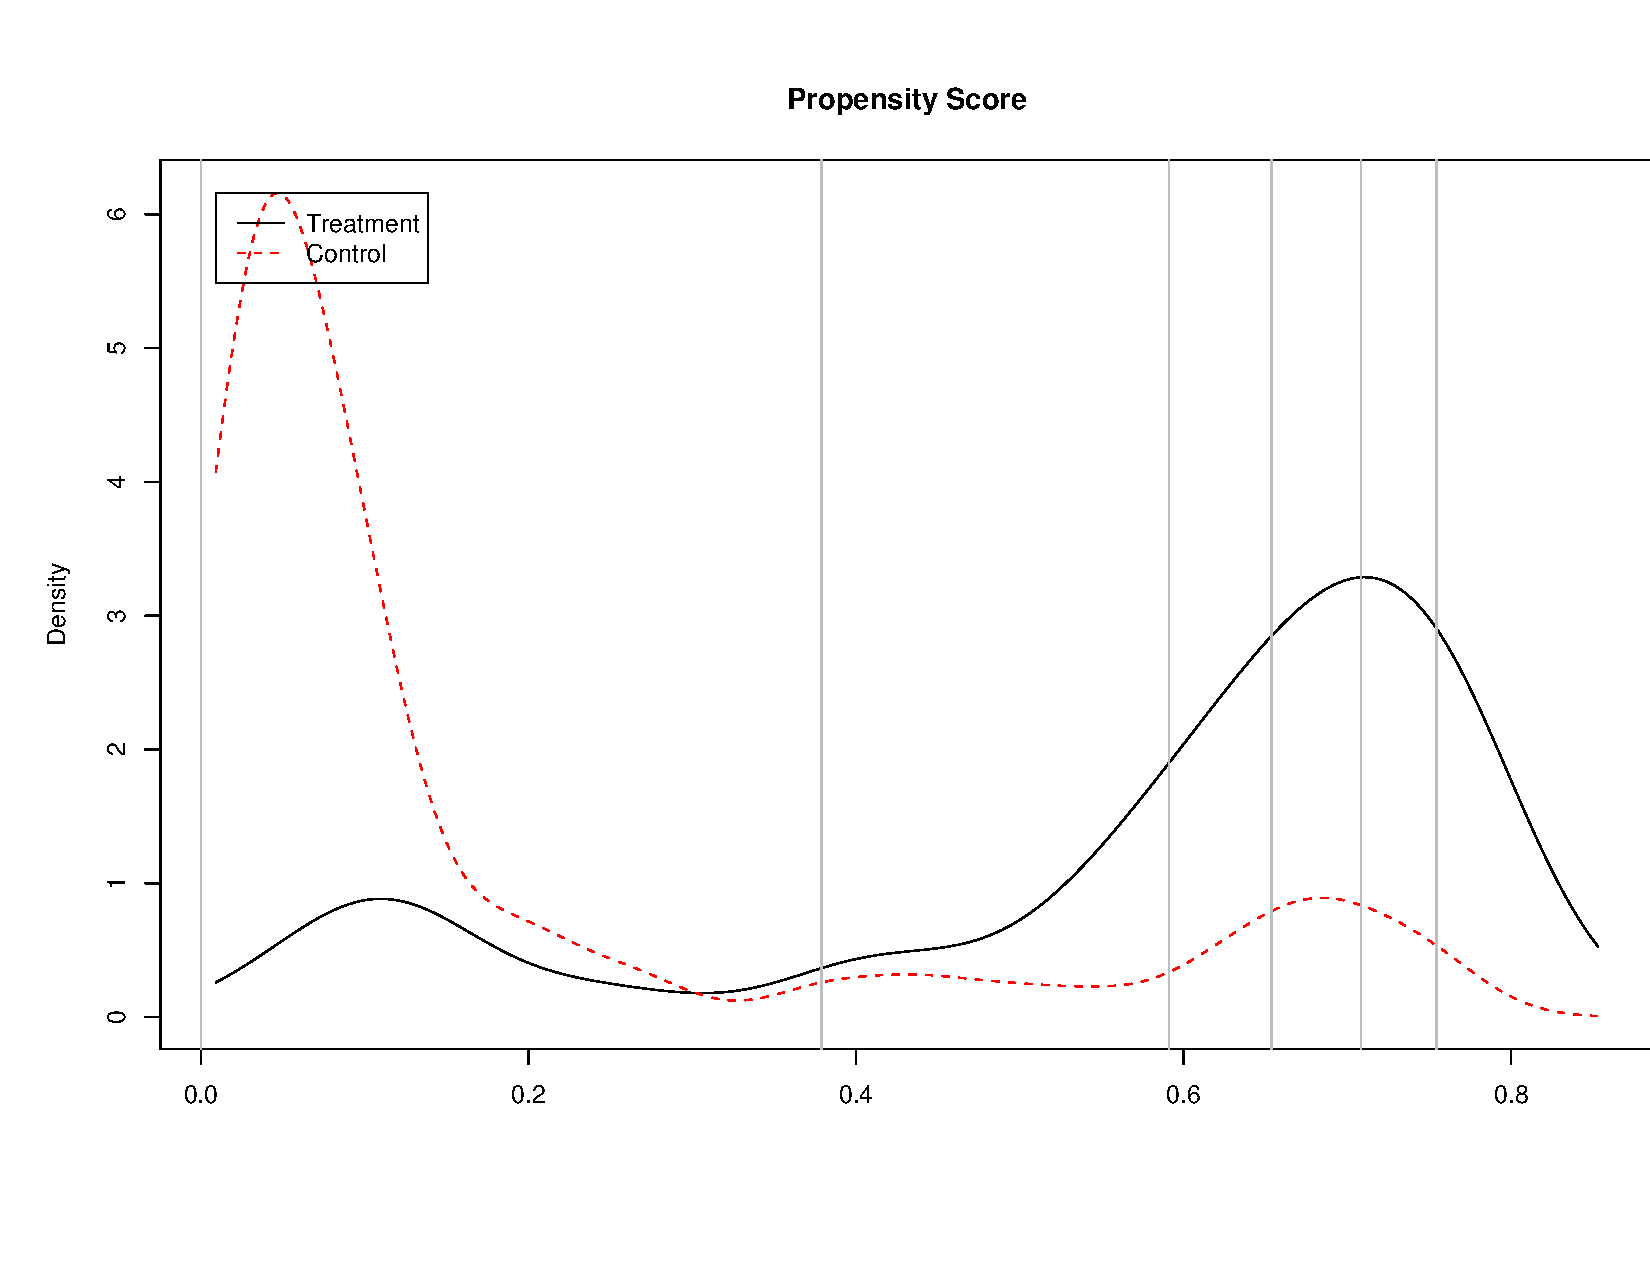
\includegraphics[height=2.85in,angle=0]{figs/subclass1}}
%    \rotatebox{270}{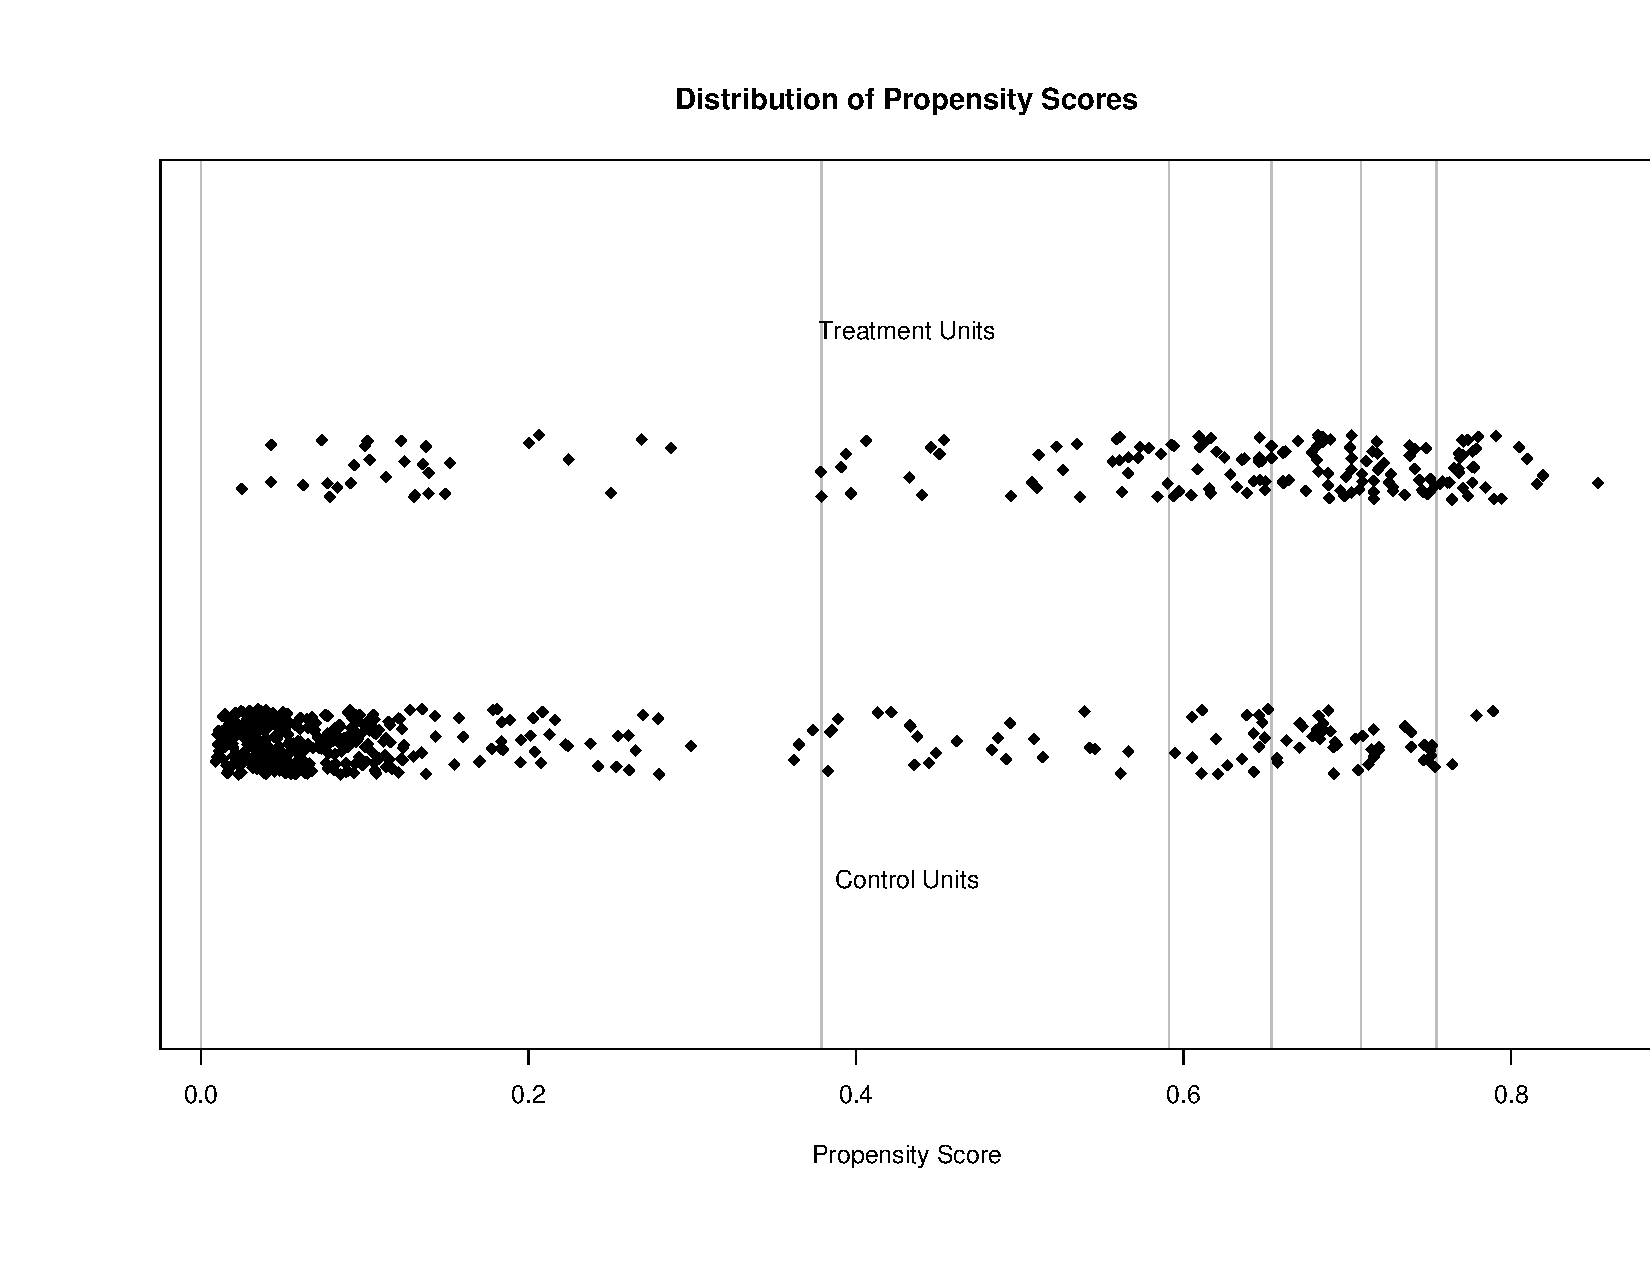
\includegraphics[height=2.85in,angle=0]{figs/subclass2}}
%    \rotatebox{270}{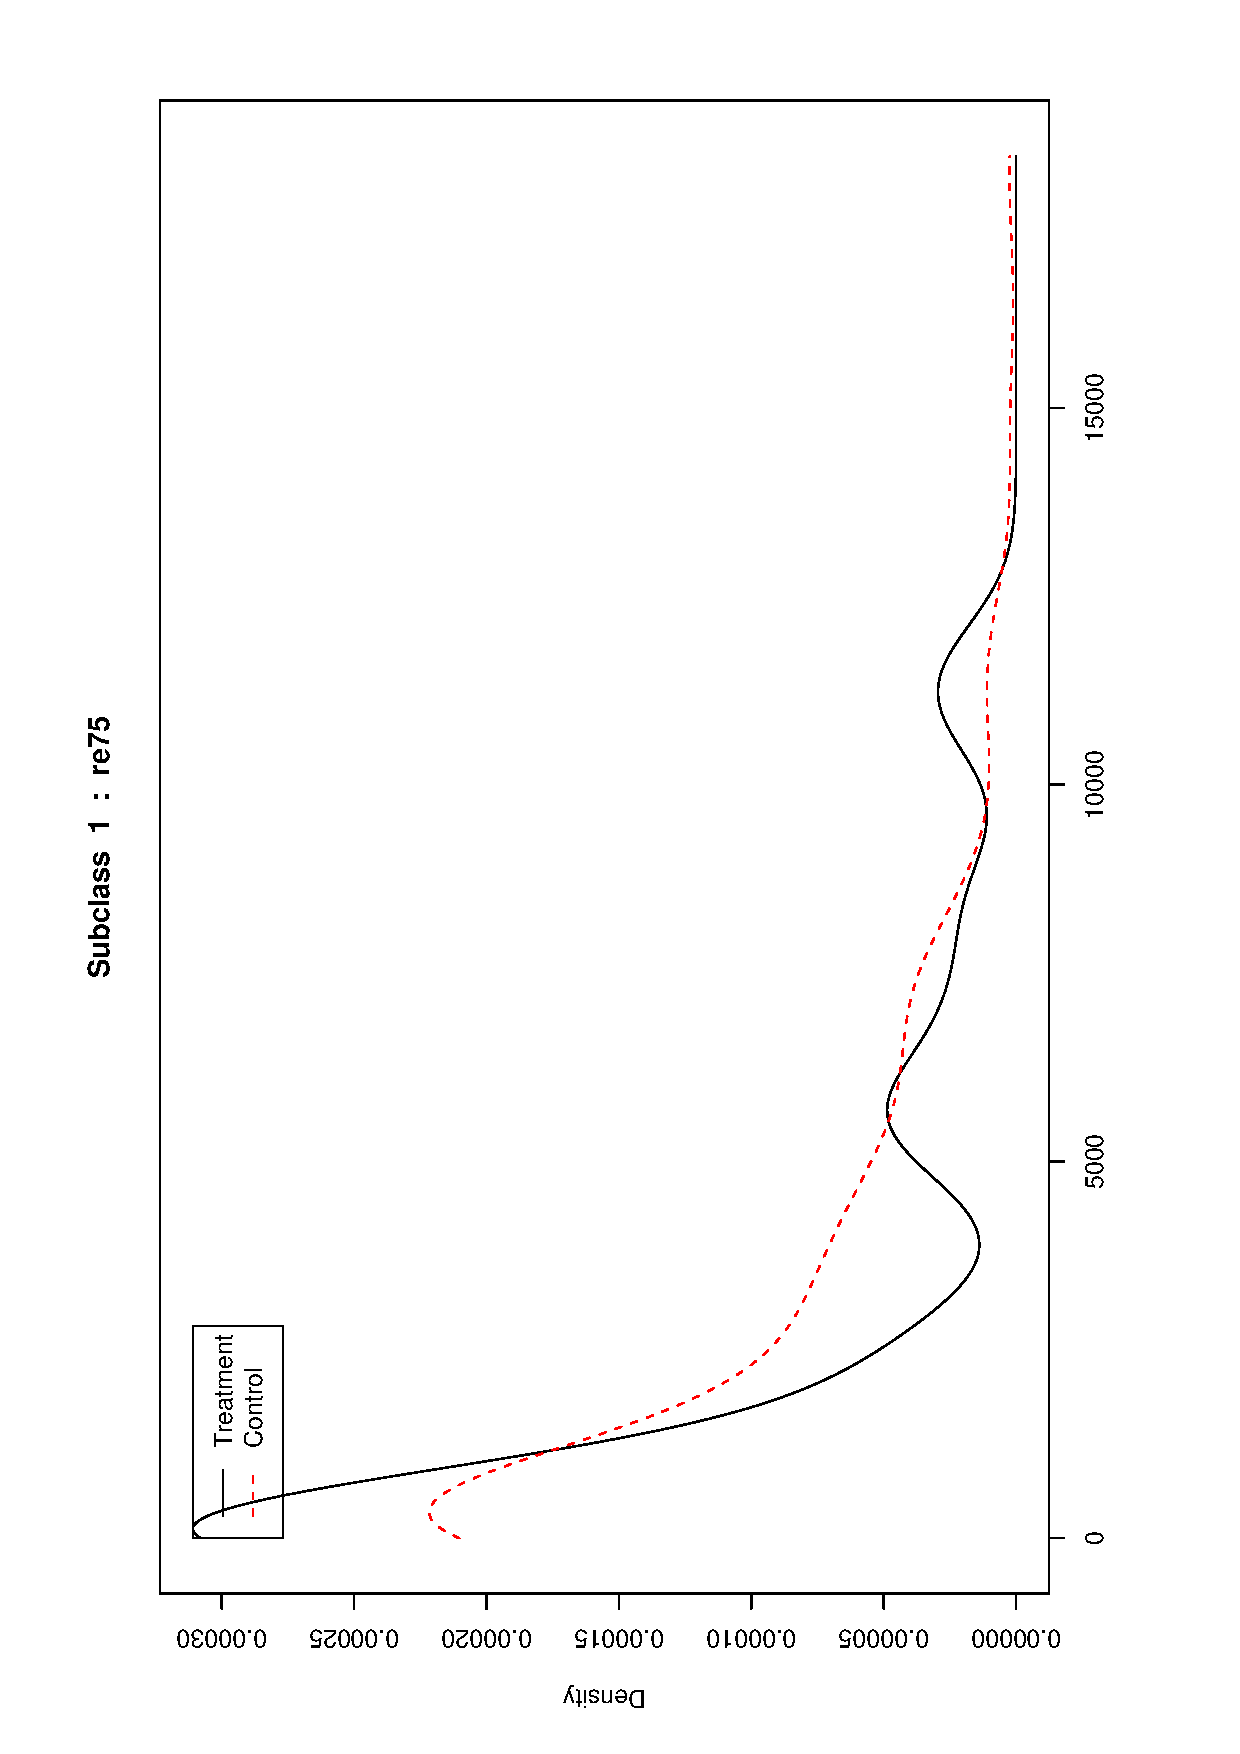
\includegraphics[height=2.85in,angle=0]{figs/subclass3}}
%    \rotatebox{270}{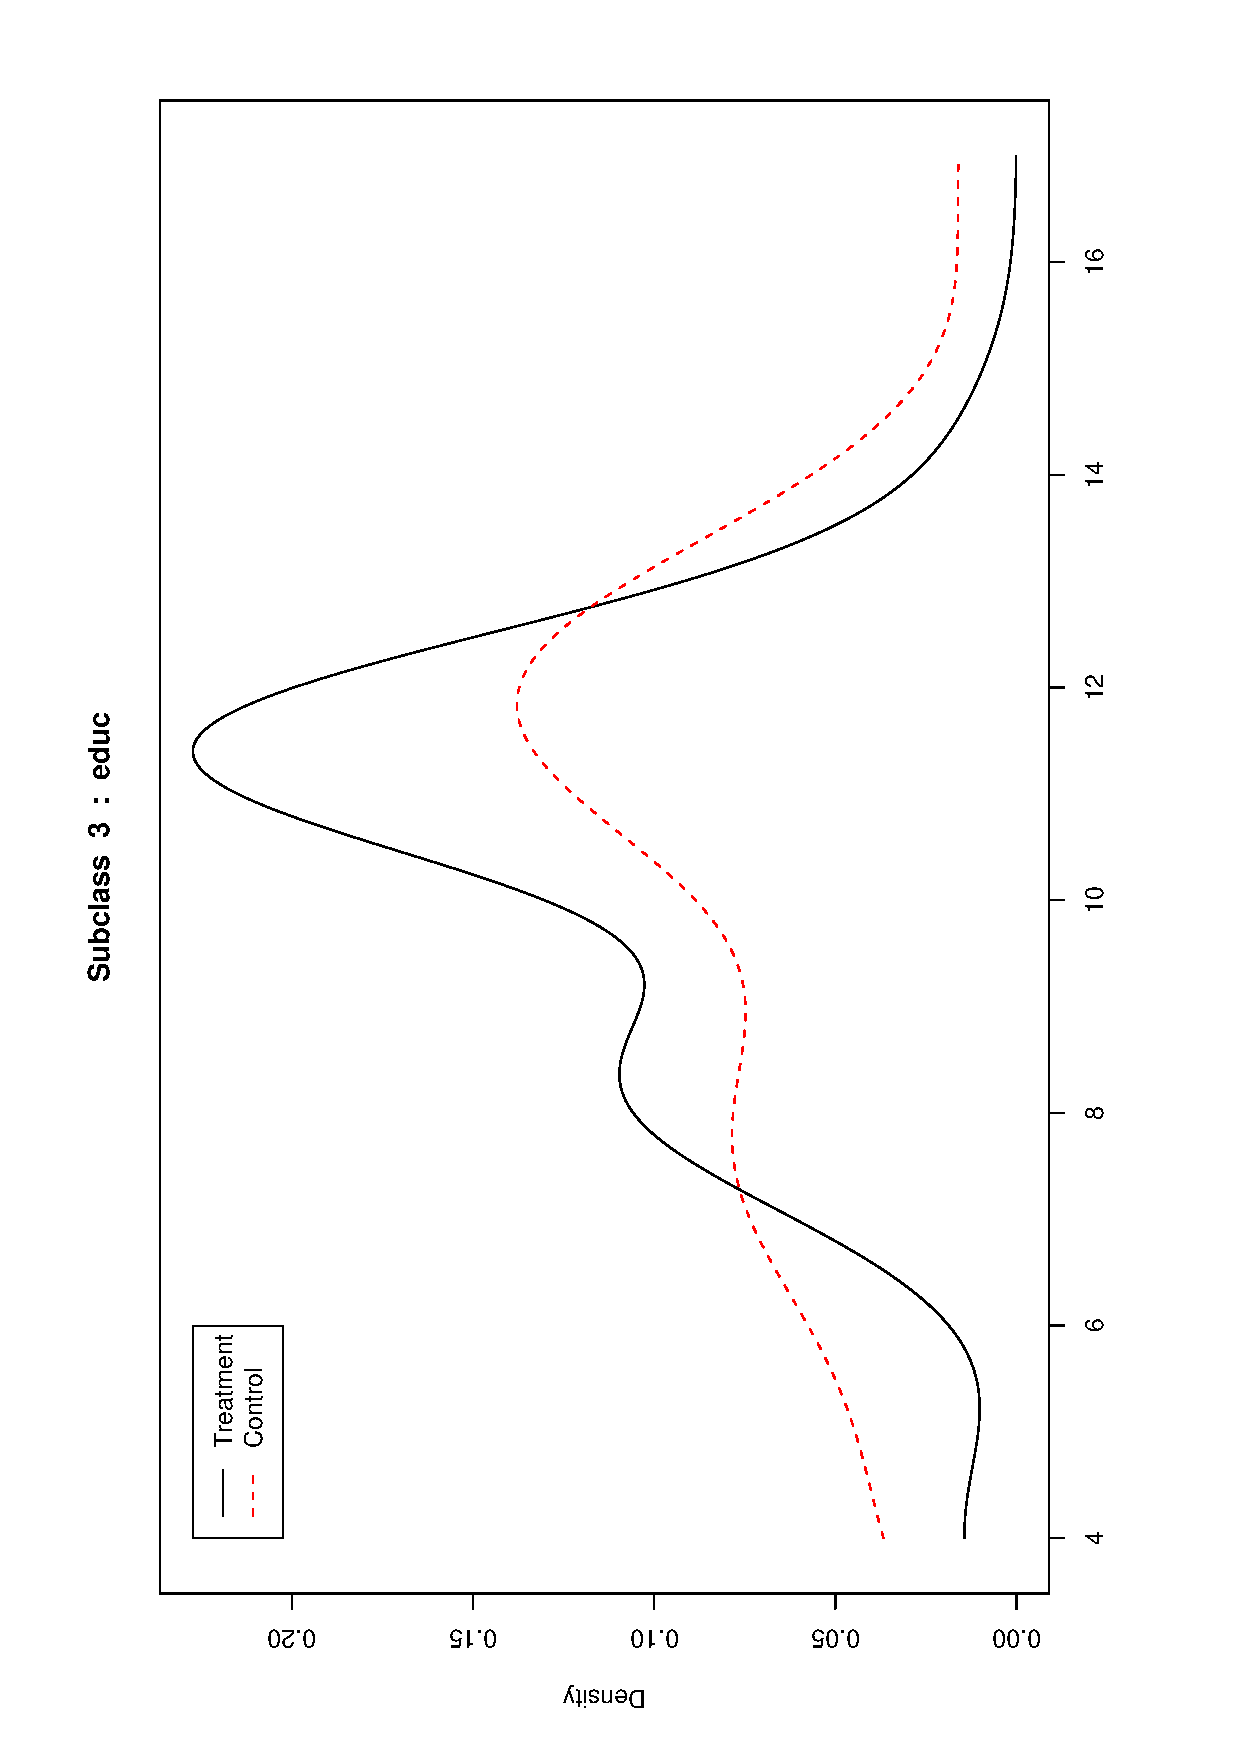
\includegraphics[height=2.85in,angle=0]{figs/subclass4}}
    {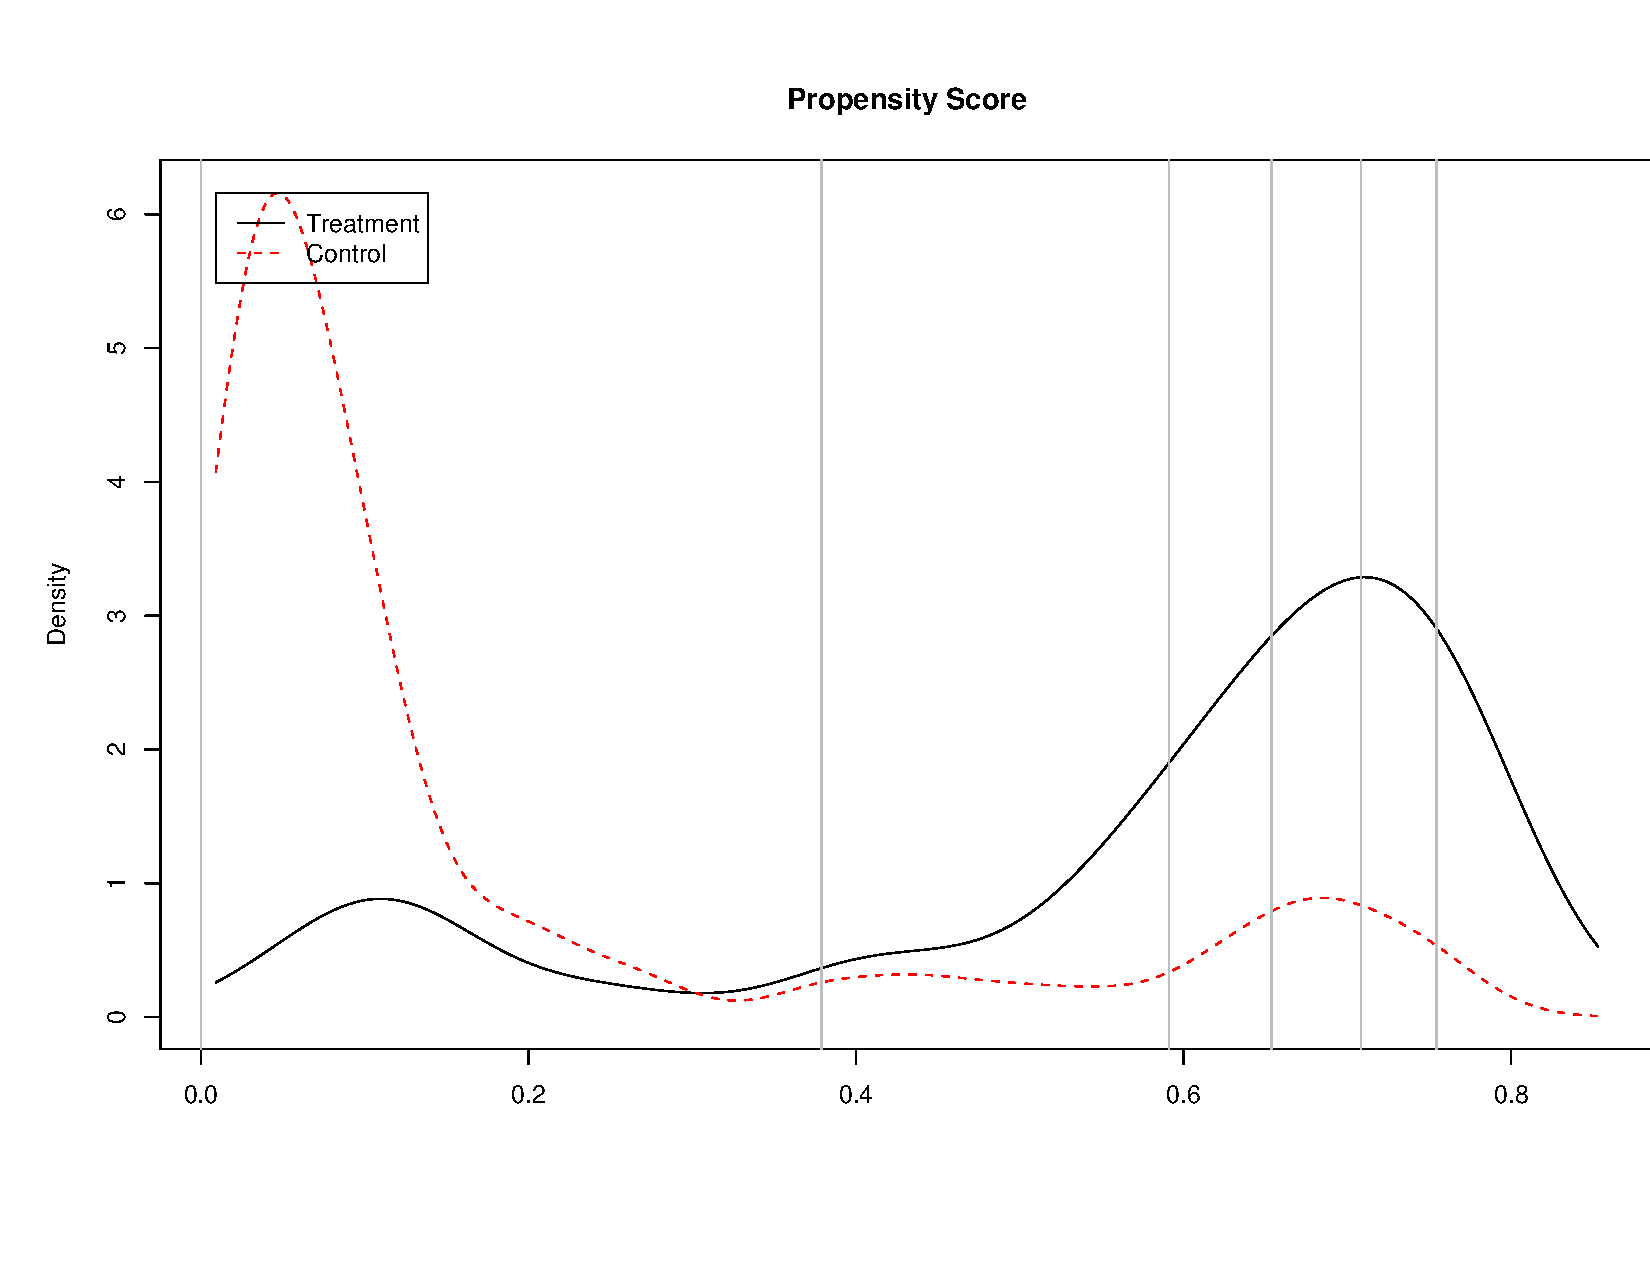
\includegraphics[scale=0.25]{figs/subclass1}}
    {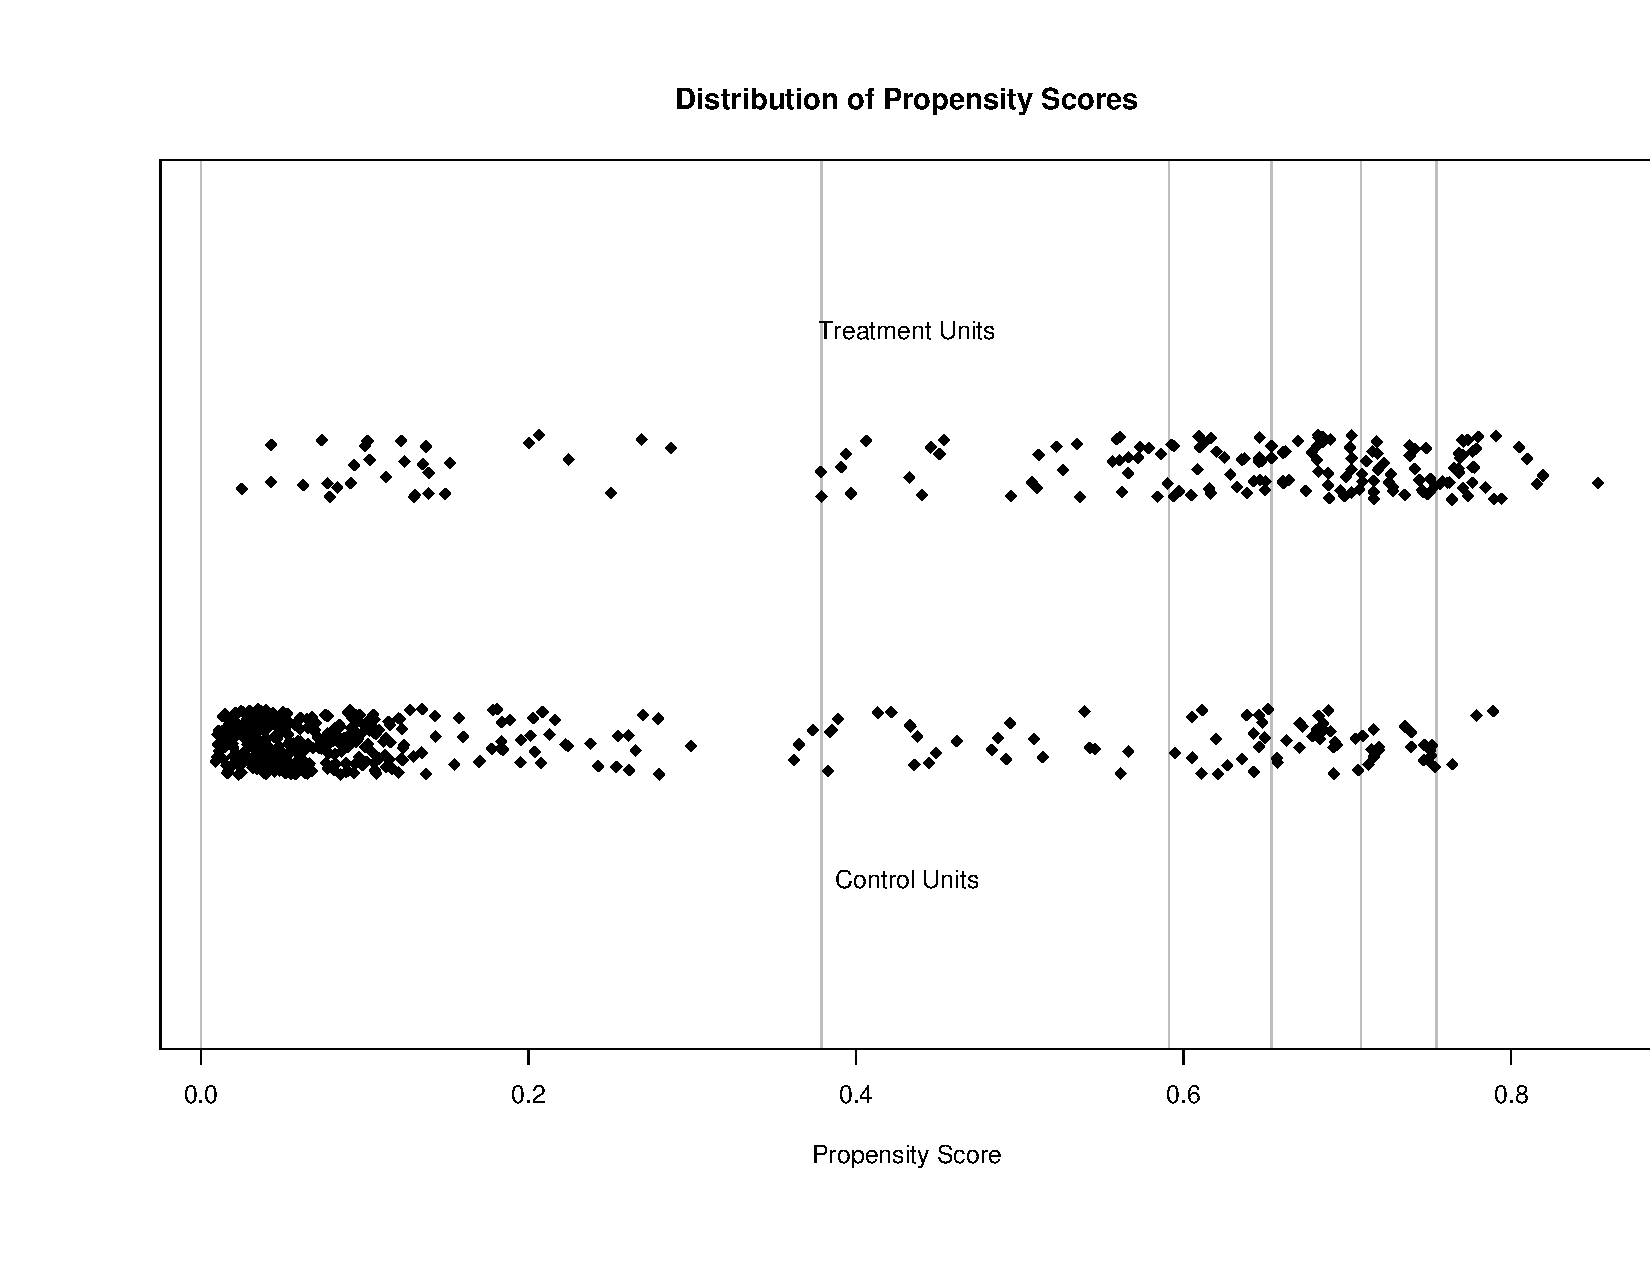
\includegraphics[scale=0.25]{figs/subclass2}}
    {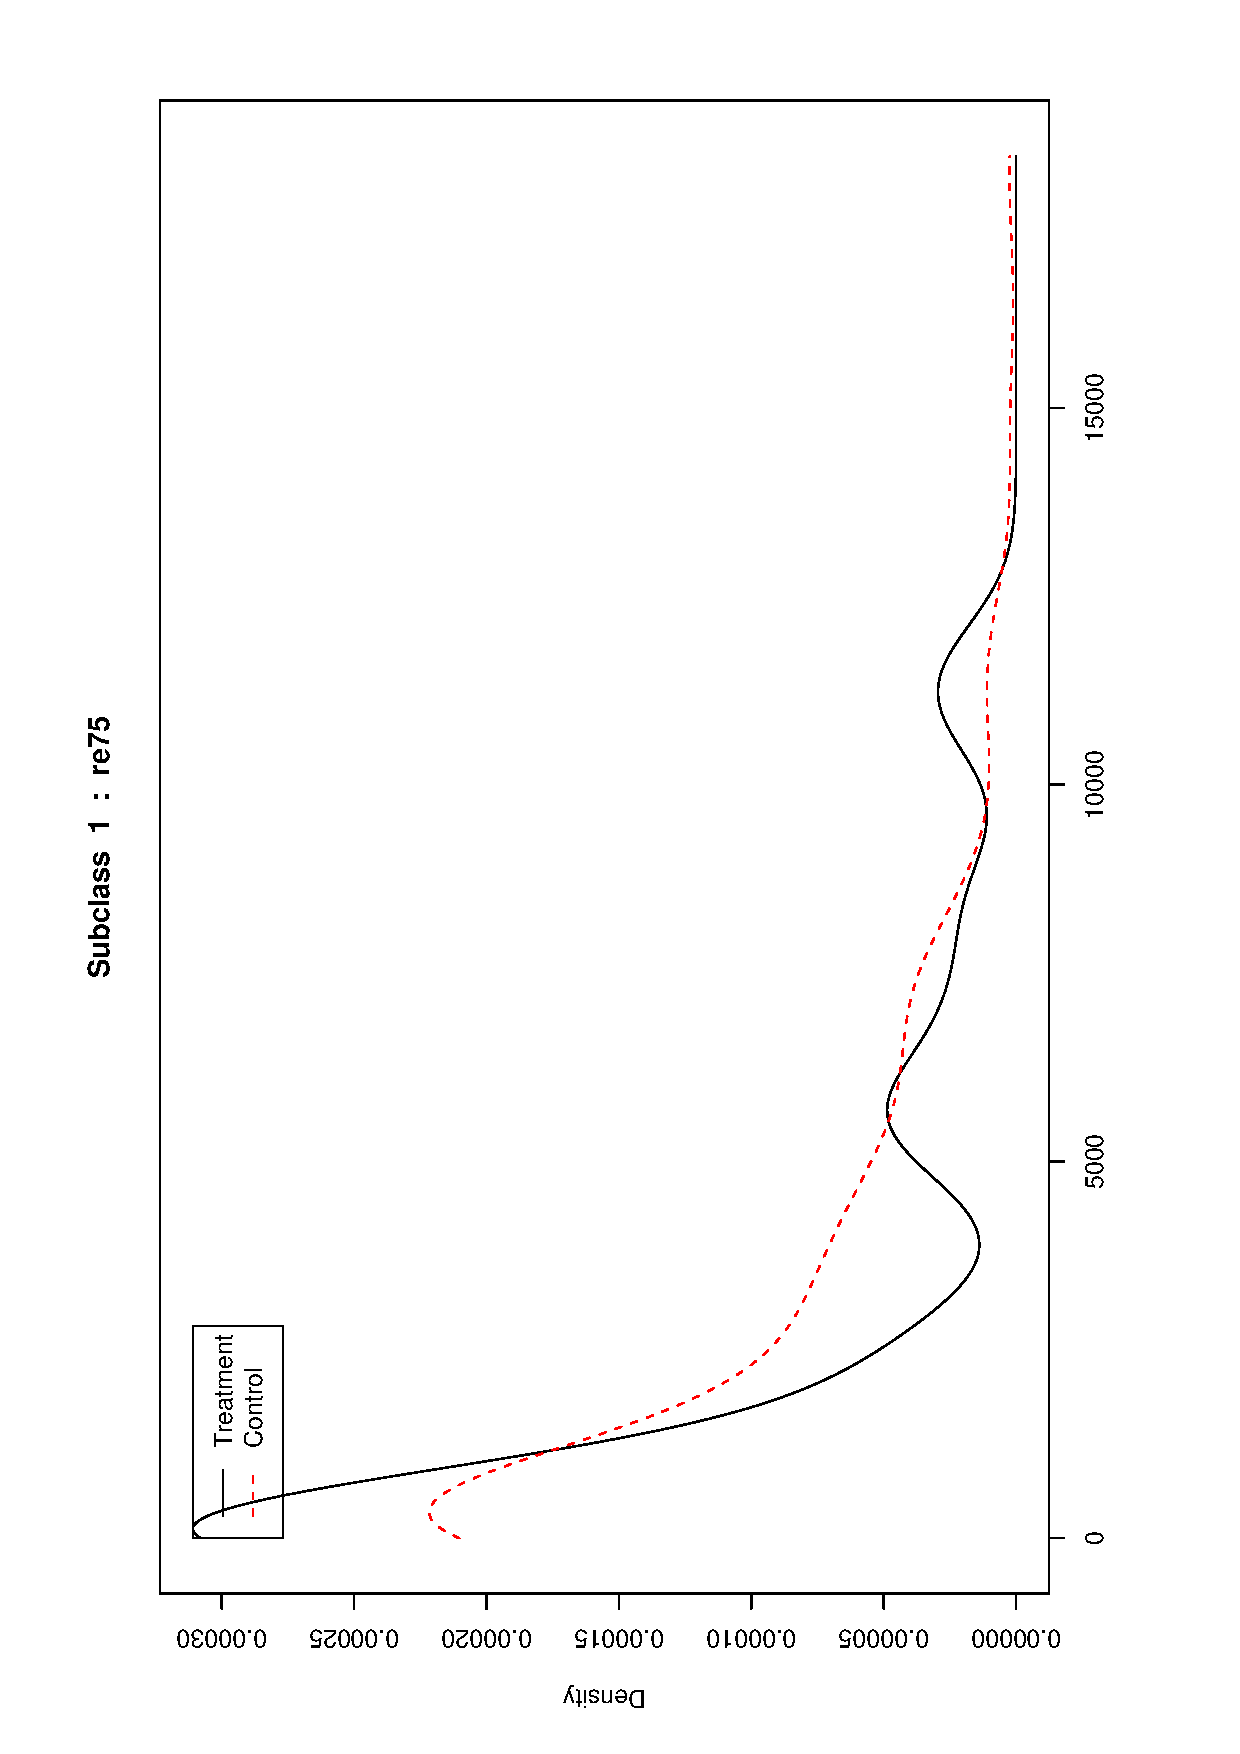
\includegraphics[scale=0.25,angle=90]{figs/subclass3}}
    {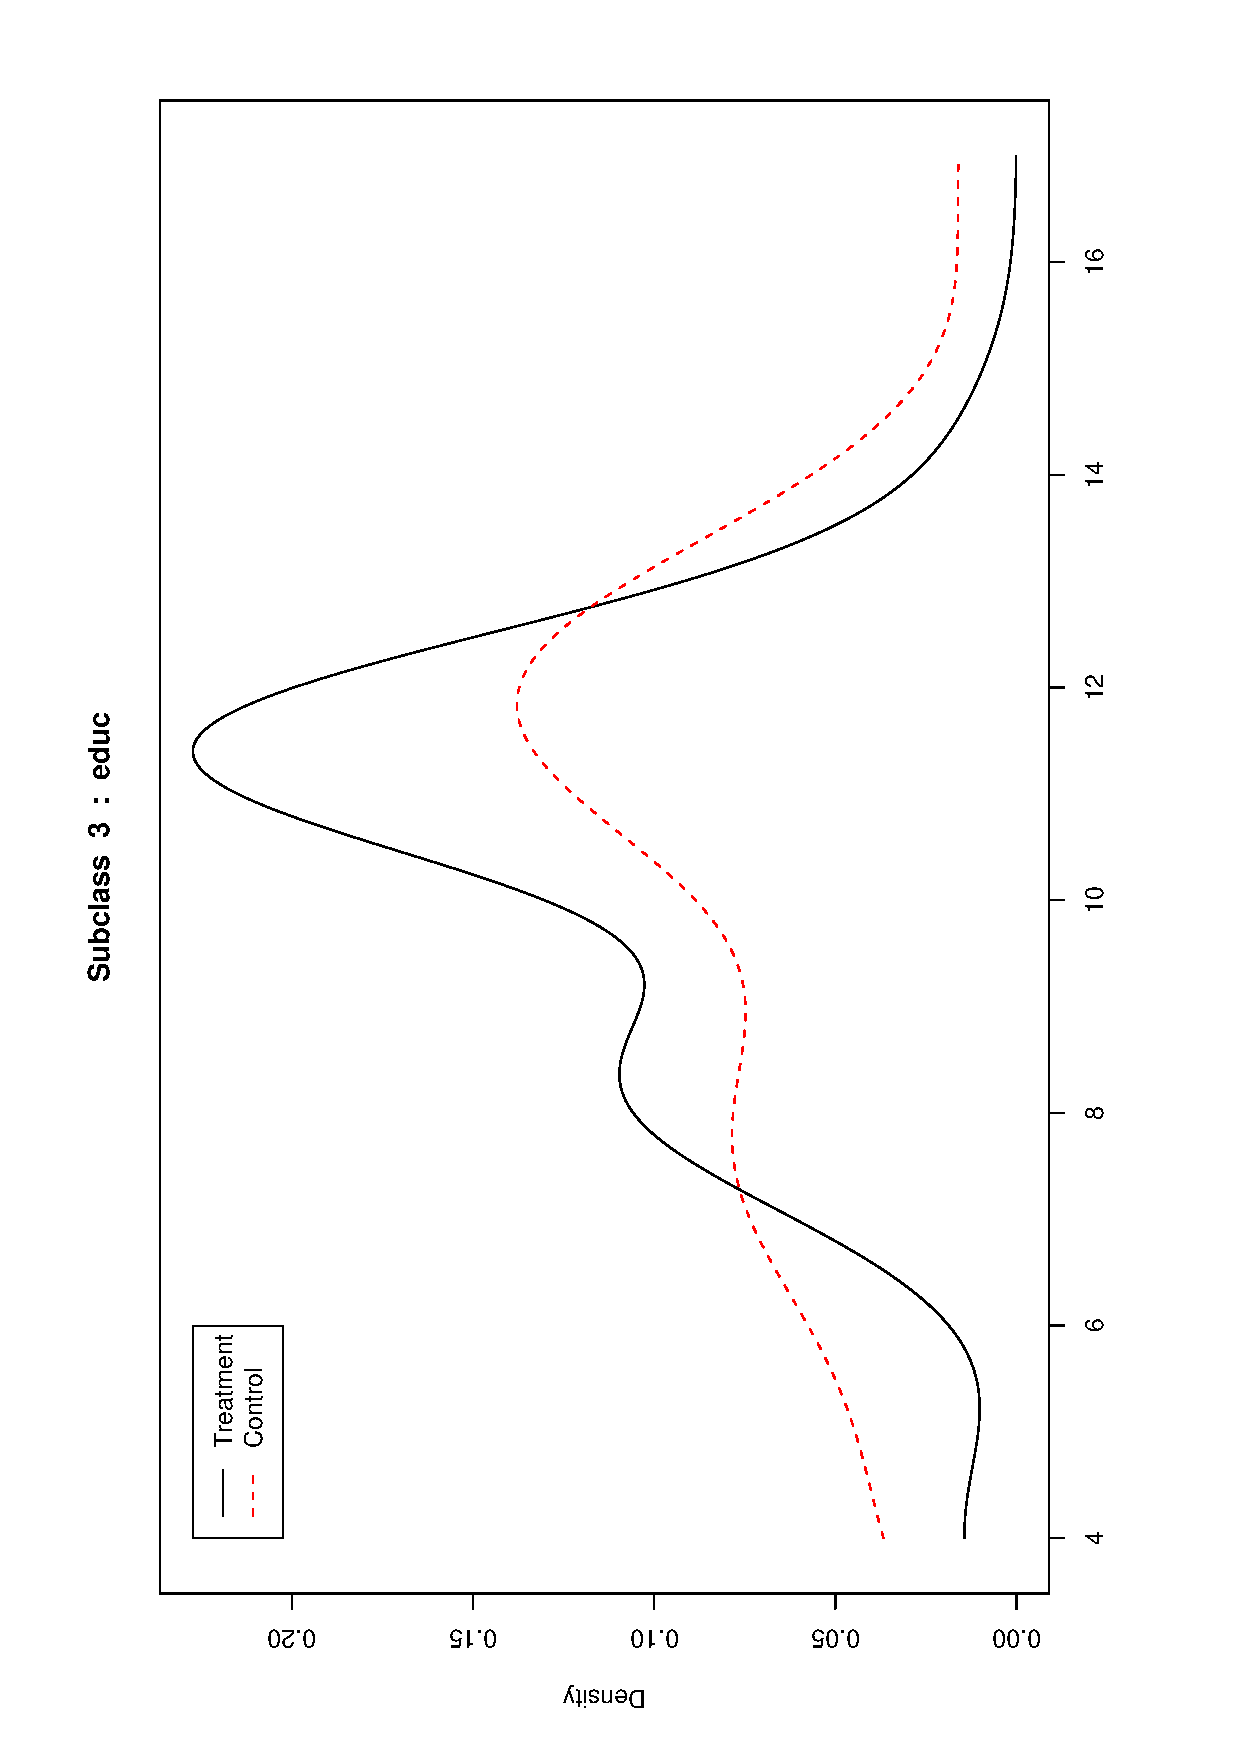
\includegraphics[scale=0.25]{figs/subclass4}}
    \hfill
    \caption{Sample interactive diagnostic graphs from \texttt{demo(lalonde)}}
\label{diags}
\end{center}
\end{figure}
\end{comment}

\subsection{Full Matching}
\label{fullmatching}

When one wishes to use all treated and control units in the analysis,
a particular type of subclassification is called ``full matching''
\citep{Rosenbaum02, Hansen04}. In this matching procedure, the matched
sample is composed of matched sets, where each matched set contains
either one treated unit and one or more controls, or one control unit
and one or more treated units.  The only units not placed into a
subclass will be those discarded (if a \texttt{discard} option was
specified).  Full matching is optimal in terms of minimizing a
weighted average of the propensity score distances between each
treated subject and each control subject within each stratum.

\subsubsection{Examples}

The following example script can be run by typing {\tt demo(full)} at
the R prompt.

\begin{verbatim}
## load the Lalonde data
data(lalonde)
## conduct full matching using the propensity score based on logistic regression
m.out <- matchit(treat ~ age + educ + black + hispan + married + nodegree + re74 + re75, 
                 data = lalonde, method = "full", distance = "logit")
## print a short summary
print(m.out)
## balance diagnostics through statistics
summary(m.out)
## balance diagnostics through graphics
plot(m.out)
\end{verbatim}


\subsection{Nearest Neighbor Matching}
\label{nearest}

Nearest neighbor matching selects the $r$ best control matches for
each individual in the treatment group (excluding those discarded
using the \texttt{discard}) option.  The matching is done using a
distance measure such as the propensity score, and matches are chosen
for each treated unit one at a time, where at each step the control
unit not yet matched that is closest to the treated unit on the
distance measure is chosen as the match.  There are many variations on
nearest neighbor matching.  See below for the options available in
\MatchIt.

Nearest neighbor matching is implemented in \MatchIt\ using the
\texttt{method="nearest"} option.

\subsubsection{Examples}

The following example script can be run by typing {\tt
    demo(nearest)} at the R prompt.

\begin{verbatim}
## load the Lalonde data
data(lalonde)
## Nearest neighbor matching on propensity score estimated using logistic regression of
## treat on re74, re75, age, and educ.  Two matches chosen for each control unit.
m.out <- matchit(treat ~ re74 + re75 + age + educ, data = lalonde, method = "nearest", 
                 distance = "logit", ratio=2)
## balance diagnostics through statistics
summary(m.out)
## balance diagnostics through graphics
plot(m.out)

## Mahalanobis matching on re74 and re75 within nearest neighbor matching on 
## distance measure, with restriction of exact matches on married.
m.out2 <- matchit(treat ~ re74 + re75 + age + educ, data = lalonde, method = "nearest", 
                  distance = "logit", mahvars=c("re74", "re75"), exact=c("married"), 
                  caliper=.25)
print(m.out2)
## balance diagnostics through statistics
summary(m.out2)
## balance diagnostics through graphics
plot(m.out2)

## Nearest neighbor matching with discard option
m.out3 <- matchit(treat ~ re74 + re75 + age + educ, data = lalonde, method = "nearest", 
                  distance = "logit", discard="both")
print(m.out3)
## balance diagnostics through statistics
summary(m.out3)
## balance diagnostics through graphics
plot(m.out3)

## Nearest neighbor matching with replacement
m.out4 <- matchit(treat ~ re74 + re75 + age + educ, data = lalonde, method = "nearest", 
                  distance = "logit", replace=TRUE, ratio=2)
print(m.out4)
## balance diagnostics through statistics
summary(m.out4)
## balance diagnostics through graphics
plot(m.out4)

## Nearest neighbor matching followed by formation of 5 subclasses
m.out5 <- matchit(treat ~ re74 + re75 + age + educ, data = lalonde, method = "nearest", 
                  distance = "logit", subclass=5)
print(m.out5)
## balance diagnostics through statistics
summary(m.out5)
## balance diagnostics through graphics
plot(m.out5)
\end{verbatim}

\subsection{Optimal Matching}
\label{optmatch}

The default nearest neighbor matching method in \MatchIt\ is
``greedy'' matching, where the closest control match for each treated
unit is chosen one at a time, without trying to minimize a global
distance measure.  Another method, ``optimal'' matching, finds the
matched samples with the smallest average absolute 
distance between each matched pair.  With large control pools, greedy
and optimal matching may lead to very similar (or the same) sets of
matches; research \citep{GuRos93} has shown that greedy and optimal
matching generally choose the same sets of controls for the matched
samples, but that optimal matching does a better job of minimizing the
distance within each pair.  In addition, optimal
matching can be particularly helpful when there are not many
appropriate control matches for the treated units.  See \cite{GuRos93}
or \cite{Rosenbaum02} for more information on optimal matching.

\subsubsection{Examples}

The following example script can be run by typing {\tt demo(optimal)}
at the R prompt.

\begin{verbatim}
## load the Lalonde data
data(lalonde)
## optimal ratio matching using the propensity score based on logistic regression
m.out <- matchit(treat ~ re74 + re75 + age + educ, data = lalonde, method = "optimal", 
                 distance = "logit", ratio = 2)
## a short summary
print(m.out)
## balance diagnostics through statistics
summary(m.out)
## balance diagnostics through graphics
plot(m.out)
\end{verbatim}


%%%%%%%%%%%%%%%%%%%%%%%%%%%%%%%%%%%%%%%%%%%%%%%%%%%%%%%%%%%%%%%%%%%%%%%%%%%

\section{References}

\subsection{Inputs}

The main command, \texttt{matchit()}, implements a variety of matching
procedures.
\begin{verbatim}
m.out <- matchit(formula, data, method = "nearest", distance = "logit",
                 distance.options=list(), discard = "none", reestimate = FALSE, ...)
\end{verbatim}
The command takes several inputs that are common for all matching
procedures in addition to inputs specific to particular matching
procedures. There is also a standard output of \texttt{matchit()}
across all commands.  We describe both here.

\subsubsection{Inputs Common to All Matching Methods}

\begin{enumerate}
  
\item \texttt{formula} takes the usual syntax of R formula, {\tt treat
    \~\ x1 + x2}, where {\tt treat} is a binary treatment indicator
  and {\tt x1} and {\tt x2} are the pre-treatment covariates. Both the
  treatment indicator and pre-treatment covariates must be contained
  in the same data frame, which is specified as {\tt data} (see
  below).  All of the usual R syntax for formulas work here. For
  example, {\tt x1:x2} represents the first order interaction term
  between {\tt x1} and {\tt x2}, and {\tt I(x1 \^\ 2)} represents the
  square term of {\tt x1}. See {\tt help(formula)} for details.
  
\item \texttt{data} specifies the data frame containing the variables
  called in {\tt formula}.  You may find it helpful for the
  diagnostics to specify observation names in the data frame (see
  Section~\ref{rnames}).
  
\item \texttt{method} specifies a matching method. Currently,
  \texttt{exact} (exact matching), \texttt{full} (full matching),
  \texttt{nearest} (nearest neighbor matching), \texttt{optimal}
  (optimal matching), and \texttt{subclass} (subclassification) are
  available. The default is \texttt{nearest}. Note that within each of
  these matching methods, \MatchIt\ offers a variety of options.  See
  Section \ref{methods} for more details.
  
\item \texttt{distance} specifies the method used to estimate the
  distance measure. The default is logistic regression, {\tt logit}.
  Before using any of these techniques, it is best to understand the
  theoretical groundings of these techniques and to evaluate the
  results.  Most of these methods (such as logistic or probit
  regression) are estimating the propensity score, defined as the
  probability of receiving treatment, conditional on the covariates
  (\cite{RosRub83}).  The distance measures used are the predicted
  probabilities from the model (the propensity scores).  Currently,
  the following methods are available:
  \begin{enumerate}
  \item {\tt mahalanobis} computes the Mahalanobis distance measure
    ({\tt mahalanobis()} in the {\tt stats} package).
  \item binomial generalized linear models with various links ({\tt
      glm()} in the {\tt stats} package); \texttt{logit} (logistic
    link), {\tt linear.logit} (logistic link with linear propensity
    score)\footnote{The linear propensity scores are obtained by
      transforming back onto a linear scale}, \texttt{probit} (probit
    link), {\tt linear.probit} (probit link with linear propensity
    score), {\tt cloglog} (complementary log-log link), {\tt
      linear.cloglog} (complementary log-log link with linear
    propensity score), {\tt log} (log link), {\tt linear.log} (log
    link with linear propensity score), {\tt cauchit} (Cauchy CDF
    link), {\tt linear.cauchit} (Cauchy CDF link with linear
    propensity score).

  \item binomial generalized additive model with various links ({\tt
      gam()} in the {\tt mgcv} package); \texttt{GAMlogit} (logistic
    link), {\tt GAMlinear.logit} (logistic link with linear propensity
    score), \texttt{probit} (probit link), {\tt GAMlinear.probit}
    (probit link with linear propensity score), {\tt GAMcloglog}
    (complementary log-log link), {\tt GAMlinear.cloglog}
    (complementary log-log link with linear propensity score), {\tt
      GAMlog} (log link), {\tt GAMlinear.log} (log link with linear
    propensity score), {\tt GAMcauchit} (Cauchy CDF link), {\tt
      GAMlinear.cauchit} (Cauchy CDF link with linear propensity
    score). \citet{HasTib90,BecJac98} and many others discuss the
    generalized additive models.

  \item \texttt{nnet}, neural network model ({\tt nnet()} in the {\tt
      nnet} package).
    \citet{BecKinZen00,Bishop95,KinZen02,White92,Zeng99} among many
    others discuss neural networks.
  
  \item \texttt{rpart}, classification trees ({\tt rpart()} in the
    \texttt{rpart} package). \citet{BreFriOls84,RugKimMar03} and many
    others discuss classification trees.
  \end{enumerate}

\item \texttt{distance.options} specifies the optional arguments that
  are passed to the model for estimating the distance measure. The
  input to this argument should be a list.
  % ** needs more detail so a user can figure out what to do with
  % this.

  % ** why delete all the advice here?  to save space?  if so, we
  % could put it somewhere else perhaps
\item \texttt{discard} specifies whether to discard units that fall
  outside some measure of support of the distance score before
  matching, and not allow them to be used at all in the matching
  procedure.  Note that discarding units may change the quantity of
  interest being estimated.
  \begin{itemize}
  \item \texttt{none} (default) discards no units before matching.
    % Use this option when the units to be matched are substantially
    % similar, such as in the case of matching treatment and control
    % units from a field experiment that was close to (but not fully)
    % randomized (e.g., \citealt{Imai05}), when caliper matching will
    % restrict the donor pool, or when you do not wish to change the
    % quantity of interest and the parametric methods to be used
    % post-matching can be trusted to extrapolate.
  \item \texttt{both} discards all units (treated and control) that
    are outside the support of the distance measure.
    % Use this option when the units to be matched are substantially
    % different (when there is a large degree of non-overlapping
    % support on the distance score), such as in the case of measuring
    % the effect of democracy on economic growth (e.g.,
    % \citealt{KinZen04}).
  \item \texttt{control} discards only control units outside the
    support of the distance measure of the treated units.
    % Use this option when the average treatment effect on the treated
    % is of most interest and when unwilling to discard
    % non-overlapping treatment units (which would change the quantity
    % of interest), such as possibly in the case of the effect of job
    % training on those individuals that actually participated in a
    % job evaluation program or a drug study where interest is in all
    % patients treated with the drug.
  \item \texttt{treat} discards only treated units outside the support
    of the distance measure of the control units.
    % Use this option when the average treatment effect on the control
    % units is of most interest and when unwilling to discard control
    % units.
  \end{itemize}
  % ** can we add an option to discard any control units not within
  % the convex hull of the treated units?  see
  % gking.harvard.edu/whatif for the code
  
\item \texttt{reestimate} specifies whether the model for distance
  measure should be re-estimated after units are discarded. The input
  must be a logical value. The default is \texttt{FALSE}.
  % Re-estimation may be desirable for efficiency reasons, especially
  % if many units were discarded and so the post-discard samples are
  % quite different from the original samples.

\item \texttt{verbose} specifies whether or not to print out comments
  indicating the status of the matching. The input must be a logical
  value. The default is \texttt{FALSE}.
\end{enumerate}

\subsubsection{Inputs Specific to Exact Matching}

Exact matching is implemented in \MatchIt\ using \texttt{method =
  "exact"}.  Exact matching will be done on all covariates included on
the right-hand side of the \texttt{formula} specified in the \MatchIt\
call.  No \texttt{distance} option is used for exact matching, and
there are no additional options for exact matching.

\subsubsection{Inputs Specific to Subclassification}

\begin{enumerate}
\item \texttt{subclass} is either (1) a scalar, specifying the number
  of subclasses, or (2) a vector of probabilities bounded between 0
  and 1, to create quantiles of the distance measure using the units
  in the group specified by \texttt{sub.by}.  The default is
  \texttt{subclass = 6}.
\item \texttt{sub.by} specifies by what criteria to subclassify:
  \texttt{"treat"} indicates by the number of treatment units
  (default), \texttt{"control"} indicates by the number of control
  units, and \texttt{"all"} indicates by the total number of units.
\end{enumerate}

\subsubsection{Inputs Specific to Nearest Neighbor Matching}

\begin{enumerate}
\item \texttt{m.order}  specifies the order in which to match
  treatment units with control units:
  \begin{itemize}
  \item {\tt "largest"} indicates matching from the largest value of
    the distance measure to the smallest. This is the default.
  \item {\tt "smallest"} indicates matching from the smallest value of
    the distance measure to the largest.
  \item {\tt "random"} indicates matching in random order.
  \end{itemize}
\item \texttt{replace} specifies whether each control unit can be
  matched to more than one treated unit.  For matching ``with
  replacement'', \texttt{replace = TRUE}.  If each control is to be
  used as a match at most once (``without replacement''), \texttt{replace
    = FALSE}. The default is {\tt FALSE}.
\item \texttt{ratio} specifies the number of control units to match to
  each treated unit, default=1.  If matching is done without
  replacement and there are fewer control units than ratio times the
  number of eligible treated units (i.e., there are not enough control 
  units for the specified method), then the higher ratios will have
  \texttt{NA} in place of the matching unit number in
  \texttt{match.matrix}.
\item \texttt{exact} specifies variables on which to perform exact
  matching within the nearest neighbor matching.  If \texttt{exact} is
  specified, only matches that exactly match on the covariates in
  \texttt{exact} will be allowed.  Within the matches that match on
  the variables in \texttt{exact}, the match with the closest distance
  measure will be chosen.  \texttt{exact} should be entered as a
  vector of variable names (\texttt{exact = c("X1", "X2")}) that are
  names of variables in \texttt{data}.
\item \texttt{caliper} specifies the number of standard deviations of
  the distance measure within which to draw control units, default=0.
  If a caliper is specified, the matches are restricted to being
  within the caliper and a control unit within the caliper for a
  treated unit is randomly selected as the match for that treated
  unit.  If \texttt{caliper != 0}, there are two additional options:
  \begin{itemize} 
  \item \texttt{calclosest} specifies whether to take the nearest
    available match if no matches are available within the
    \texttt{caliper}. The default is {\tt FALSE}.
  \item \texttt{mahvars} specifies variables on which to perform
    Mahalanobis-metric matching within each caliper (default=NULL).
    Variables should be entered as a vector of variable names
    (\texttt{mahvars=c("X1","X2")}) that are names of variables in
    \texttt{data}.  If \texttt{mahvars} is specified without
    \texttt{caliper}, the caliper is set to 0.25.
  \end{itemize}
\item \texttt{subclass} and \texttt{sub.by}.  See Section
  \ref{subclass} for more details on these options.  If a
  \texttt{subclass} is specified within \texttt{method = "nearest"},
  the matched units will be placed into subclasses after the nearest
  neighbor matching is completed.
\end{enumerate}


\subsubsection{Inputs Specific to Full Matching}

Full matching can be performed with \MatchIt\ by setting
\texttt{method = "full"}.  We use an add-on package called
\texttt{optmatch} \citep{Hansen04}, which must be installed separately
by typing at the R command prompt,
\begin{verbatim}
install.packages("optmatch", contriburl = "http://www.stat.lsa.umich.edu/~bbh/optmatch")
\end{verbatim}
For more information about the package, see
\hlink{http://www.stat.lsa.umich.edu/\~{}bbh/optmatch.html}{http://www.stat.lsa.umich.edu/\~bbh/optmatch.html}.
The available options are listed below.

\begin{enumerate}
\item {\tt ...} represents additional inputs that can be passed to the
  {\tt fullmatch()} function in the {\tt optmatch} package. See {\tt
    help(fullmatch)} for details.
\end{enumerate}

\subsubsection{Inputs Specific to Optimal Matching}

Optimal matching is performed with \MatchIt\ by setting \texttt{method
  = "optimal"}.  We use an add-on package called \texttt{optmatch}
\citep{Hansen04}, which must be installed separately by typing at the
R command prompt,
%** can we do this automatically if its needed?
\begin{verbatim}
install.packages("optmatch", contriburl = "http://www.stat.lsa.umich.edu/~bbh/optmatch")
\end{verbatim}
Currently, \texttt{optmatch} is only available for Unix and MacOS X
(but not for Windows).  For more information about the package, see
\hlink{http://www.stat.lsa.umich.edu/\~{}bbh/optmatch.html}{http://www.stat.lsa.umich.edu/\~bbh/optmatch.html}.
The available options are listed below.

\begin{enumerate}
\item {\tt ratio} specifies the number of control units to be matched
  to each treatment unit, the default is {\tt 1}.
\item {\tt ...} represents additional inputs that can be passed to the
  {\tt fullmatch()} function in the {\tt optmatch} package. See {\tt
    help(fullmatch)} for details.
\end{enumerate}



%%%%%%%%%%%%%%%%%%%%%%%%%%%%%%%%%%%%%%%%%%%%%%%%%%%%%%%%%%%%%%%%%%%%%%

\subsection{Outputs}

\subsubsection{Output Object Contents}

The following are the elements of the \texttt{matchit} output object;

\begin{enumerate}
\item \texttt{call} provides the original {\tt matchit()} call.
  
\item \texttt{formula} shows the formula used to specify the model for
  estimating the distance measure.
  
\item \texttt{model} stores the output of the model used to estimate
  the distance measure.  \texttt{summary(m.out\$model)} will give the
  summary of the model where \texttt{m.out} is the output object from
  \texttt{matchit()}.
  
  % ** n_1 and ratio aren't defined at this point so its hard to
  % follow what the next line means, even with the subsequent list.
\item \texttt{match.matrix} is an $n_1$ by \texttt{ratio} matrix
  where:
  \begin{itemize}
  \item the row names, which can be obtained through
    \texttt{row.names(match.matrix)}, represent the names of the
    treatment units, which come from the data frame specified in
    \texttt{data} (to learn how to do this, see Section~\ref{rnames}).
  \item each column stores the name(s) of the control unit(s) matched
    to the treatment unit of that row. For example, when the
    \texttt{ratio} input for nearest neighbor or optimal matching is
    specified as 3, the three columns of \texttt{match.matrix}
    represent the three control units matched to one treatment unit).
  \item \texttt{NA} indicates that the treatment unit was not matched.
  \end{itemize}
   
\item \texttt{discarded} is a vector of length $n$ that displays
  whether the units were ineligible for matching due to common support
  restrictions.  It equals \texttt{TRUE} if unit $i$ was discarded,
  and it is set to \texttt{FALSE} otherwise.
  
\item \texttt{distance} is a vector of length $n$ with the estimated
  distance measure for each unit.
  
\item \texttt{weights} is a vector of length $n$ that provides the
  weights assigned to each unit in the matching process.  Unmatched
  units have weights equal to $0$. Matched treated units have weight
  $1$.  Each matched control unit has weight proportional to the
  number of treatment units to which it was matched, and the sum of
  the control weights is equal to the number of uniquely matched
  control units. See Section~\ref{subsec:weights} for more details.
  
\item \texttt{subclass} contains the subclass index in an ordinal
  scale from 1 to the total number of subclasses as specified in
  \texttt{subclass} (or the total number of subclasses from full or
  exact matching).  Unmatched units have \texttt{NA}.
  
\item \texttt{q.cut} gives the subclass cut-points that classify the
  distance measure.
  
\item \texttt{treat} stores the treatment indicator from \texttt{data}
  (the left-hand side of \texttt{formula}).
 
\item \texttt{X} stores the covariates used for estimating the
  distance measure (the right-hand side of \texttt{formula}).
\end{enumerate}


\subsubsection{{\tt summary()}}
The \texttt{summary} command returns more information about the
\MatchIt\ model.  Optional inputs are:

\begin{enumerate}
\item \texttt{interactions}, which is an option to calculate summary
  statistics in \texttt{sum.all} and \texttt{sum.matched} for all
  covariates, their squares, and two-way interactions when
  \texttt{interactions=TRUE} and only the covariates themselves when
  \texttt{interactions=FALSE} (default).
\item \texttt{addlvariables}, which may contain additional variables
  on which to calculate the diagnostic statistics (in addition to the
  variables included in the matching procedure).  By default,
  \texttt{addlvariables=NULL}.  \texttt{addlvariables} must be
  specified as a data frame, with the same number of units and units
  in the same order as in the data set sent to \MatchIt .
\end{enumerate}

The \texttt{summary} call returns, when applicable:

\begin{enumerate}
\item The original assignment model call.
\item \texttt{sum.all} is a data frame that contains variable names
  and interactions down the row names, and summary statistics on
  \emph{all observations} in each of the columns.  The columns in
  \texttt{sum.all} contain \footnote{The values output for full
    matching are slightly different from that described here; see
    Section \ref{fullmatching} for details}:
  \begin{itemize}
  \item means of all covariates $X$ for treated and control units,
    where \texttt{Means Treated}$= \mu_{X|T=1} = \frac{1}{n_1}
    \sum_{T=1} X_i$ and \texttt{Means Control}$= \mu_{X|T=0} =
    \frac{1}{n_0} \sum_{T=0} X_i$,
  \item pooled standard deviations for all covariates $X$, where ${\rm
      SD} = s_X = \sqrt{\frac{1}{n-1} \sum_{i} (X_i -
      \overline{X})^2}$.
  \item summary statistics from a Q-Q plot, which compares treated and
    control covariate distributions, where \texttt{QQ Med}, \texttt{QQ
      Mean}, and \texttt{QQ Max} indicate the median, mean, and
    maximum orthogonal deviations from the 45 degree line of a Q-Q
    plot.
  \item standardized bias statistics, $${\rm Std.
      Bias}=\frac{\mu_{X|T=1} - \mu_{X|T=0}}{s_{x|T=1}}, \quad {\rm
      where} \quad s_{x|T=1} = \sqrt{\frac{\sum_{i \in \{i: T_i=1\}}
        X_i - \mu_{X|T=1}}{n_1-1} }.$$
  \end{itemize}
  
\item \texttt{sum.matched} is a data frame which contains variable
  names down the row names, and summary statistics on only the
  \emph{matched observations} in each of the columns.  Specifically,
  the columns in \texttt{sum.matched} contain the following
  elements\footnote{The values output for full matching are slightly
    different from that described here; see Section \ref{fullmatching}
    for details}:
  \begin{itemize}
  \item weighted means for matched treatment units of all covariates
    $X$ and their interactions, where \texttt{Means Treated}$=
    \mu_{wX|T=1} = \frac{1}{n_1} \sum_{T=1} w_iX_i$ and \texttt{Means
      Control}$=\mu_{wX|T=0} = \frac{1}{n_0} \sum_{T=0} w_iX_i$,
  \item weighted standard deviations for all covariates $X$ and their
    interactions of matched units, where \texttt{SD} $= s_{wX} =
    \sqrt{\frac{1}{n} \sum_{i} (w_iX_i - \overline{X}^*)^2}$, where
    $\overline{X}^*$ is the weighted mean of $X$.
  \item standardized bias statistics \texttt{Std.
      Bias}$=\frac{\mu_{wX|T=1} - \mu_{wX|T=0}}{s_{x|T=1}}$, and
  \end{itemize}
  where $w$ represents the vector of \texttt{weights}.
  
\item \texttt{reduction} shows the percent bias reduction achieved in
  each of the balance measures in \texttt{sum.all} and
  \texttt{sum.matched}, defined as $100(|a|-|b|)/|a|$, where $a$ was
  the value of the balance measure before matching and $b$ is the
  value of the balance measure after matching.

\item \texttt{nn} gives the sample sizes in the full and matched
  samples and the number of discarded units, by treatment and control.
  
\item \texttt{q.table} is an array that contains the same information
  as \texttt{sum.matched} by subclass.
  
\item \texttt{qn} gives the sample sizes in the full and matched
  samples and the number of discarded units, by subclass and by
  treatment and control.
\item \texttt{match.matrix} from the {\texttt matchit} output.
\end{enumerate}

\subsubsection{{\tt plot()}}

The \texttt{plot} command allows you to check the distributions of
covariates in the assignment model, squares, and interactions, and
within each subclasses if specified.  The graphs present:
\begin{enumerate}
\item Jitter plots of the propensity score for treated and control
  units (\texttt{type="jitter}).
\item Q-Q plots of each covariate to check balance of marginal
  distributions.  This graph plots covariate values that fall in
  (approximately) the same quantile of treated and control
  distributions.  Control unit quantile values are plotted on the
  x-axis, and treated unit quantile values are plotted on the y-axis.
  If values fall below the 45 degree line, control units generally
  take lower values of the covariate.  Data points that fall exactly
  on the 45 degree line indicate that the marginal distributions are
  identical.  Discrete covariates that take 5 or fewer values are
  jittered for visibility.  This may be changed by setting the option
  \texttt{discrete.cutoff} (\texttt{type="QQ"} (default)).
\end{enumerate}

\subsubsection{Examples}
The following is an example of the output from using
\texttt{summary()} on an output object from {\tt matchit()} generated
using nearest neighbor matching, followed by sample plots from
\texttt{plot()}:

\begin{verbatim}

> m.out <- matchit(treat ~ re74 + re75 + educ + black + hispan + age, data = lalonde, 
                   method = "nearest")
 
> print(summary(m.out))

Call:
matchit(formula = treat ~ re74 + re75 + educ + black + hispan + age, data = lalonde, 
method = "nearest")

Summary of balance for all data:

         Means Treated Means Control Pooled SD   QQ Med  QQ Mean   QQ Max Std. Bias
distance      5.66e-01         0.187     0.284    0.732    0.535     0.84     1.792 
re74          2.10e+03      5619.237  6477.964 3430.277 5155.851 13044.16    -0.721
re75          1.53e+03      2466.484  3295.679 1373.280 1511.706  9609.60    -0.290
educ          1.03e+01        10.235     2.628    1.414    0.962     5.66     0.055
black         8.43e-01         0.203     0.489    1.414    0.903     1.41     1.757
hispan        5.95e-02         0.142     0.322    0.000    0.119     1.41    -0.349
age           2.58e+01        28.030     9.881    1.414    4.650    14.14    -0.309
        
Summary of balance for matched data:

         Means Treated Means Control Pooled SD  QQ Med QQ Mean   QQ Max Std. Bias
distance      5.66e-01         0.365     0.257   0.150   0.284 6.93e-01    0.9509
re74          2.10e+03      2466.304  4574.949 410.082 978.726 1.86e+04   -0.0759
re75          1.53e+03      1960.355  3089.993 638.038 887.982 1.61e+04   -0.1330
educ          1.03e+01        10.470     2.673   1.414   1.307 5.66e+00   -0.0618
black         8.43e-01         0.470     0.475   0.000   0.527 1.41e+00    1.0231
hispan        5.95e-02         0.276     0.374   0.000   0.306 1.41e+00   -0.9118
age           2.58e+01        26.054     8.794   2.828   3.868 1.13e+01   -0.0332
        
Percent Balance Improvement:

           Mean QQ Med QQ Mean QQ Max Std. Bias
distance   46.9   79.4    46.8   17.6      46.9
re74       89.5   88.0    81.0  -42.3      89.5
re75       54.2   53.5    41.3  -67.3      54.2
educ      -12.5    0.0   -35.9    0.0     -12.5
black      41.8  100.0    41.6    0.0      41.8
hispan   -161.3    0.0  -157.7    0.0    -161.3
age        89.3 -100.0    16.8   20.0      89.3

Sample sizes:

          Control Treated
Full          429     185
Matched       185     185
Unmatched     244       0
Discarded       0       0

\end{verbatim}

For this 1:1 nearest neighbor matching, we see that 185 control units
were matched to the 185 treatment units.  The \texttt{summary()}
command first gives measures of the balance between the treated and
control groups in the full (original) data set, and then the same
measures of balance in the matched data set.  If the matching worked
well, the standardized bias and QQ plot statistics should be smaller
in the matched data set as compared with the full data set.  We could
also use the \texttt{addlvars} option to examine the balance in
variables not included in the distance model; it may be beneficial to
include in the distance model any variables that are not well balanced
in the matched data sets.

We can also examine the balance graphically:

\begin{verbatim}
> plot(m.out)
> plot(m.out, type="jitter")
\end{verbatim}

\begin{figure}[tbp]
  \begin{center}
%    \rotatebox{270}{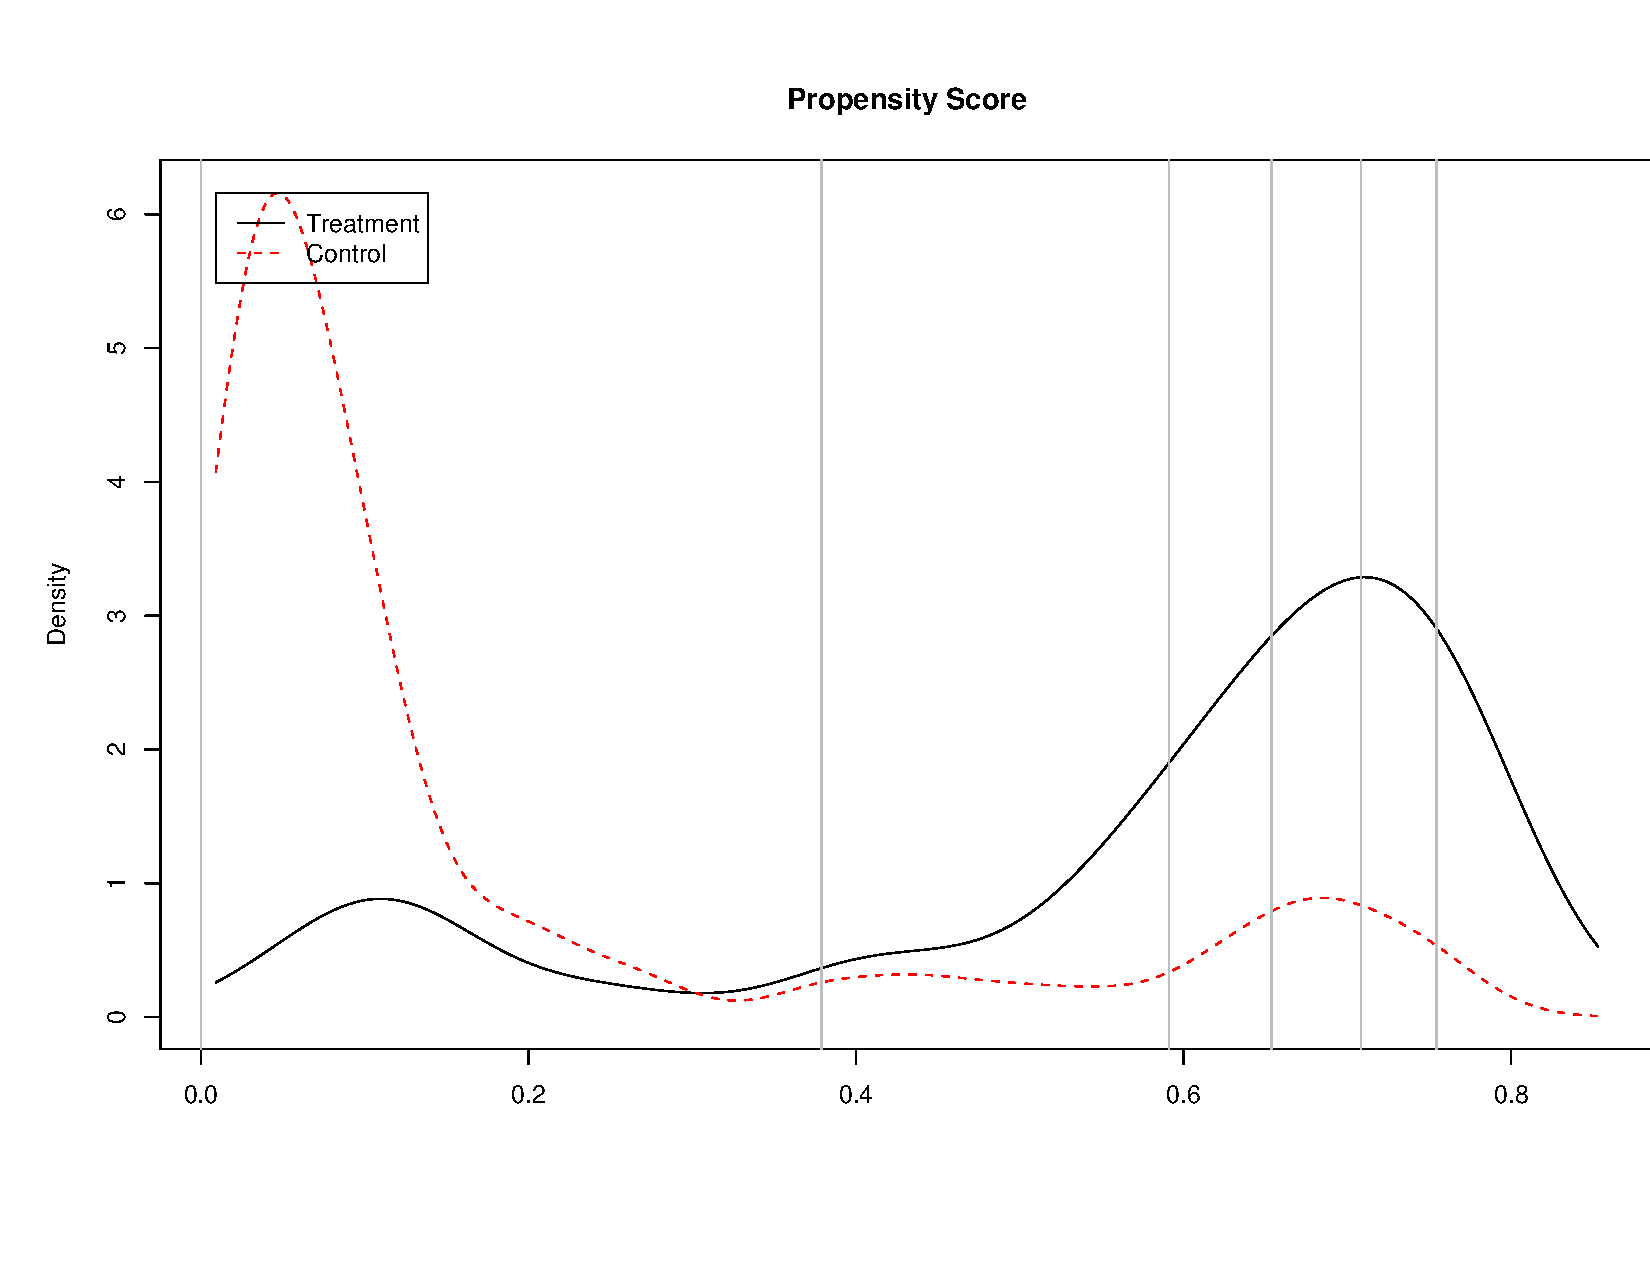
\includegraphics[height=2.85in,angle=0]{figs/subclass1}}
    {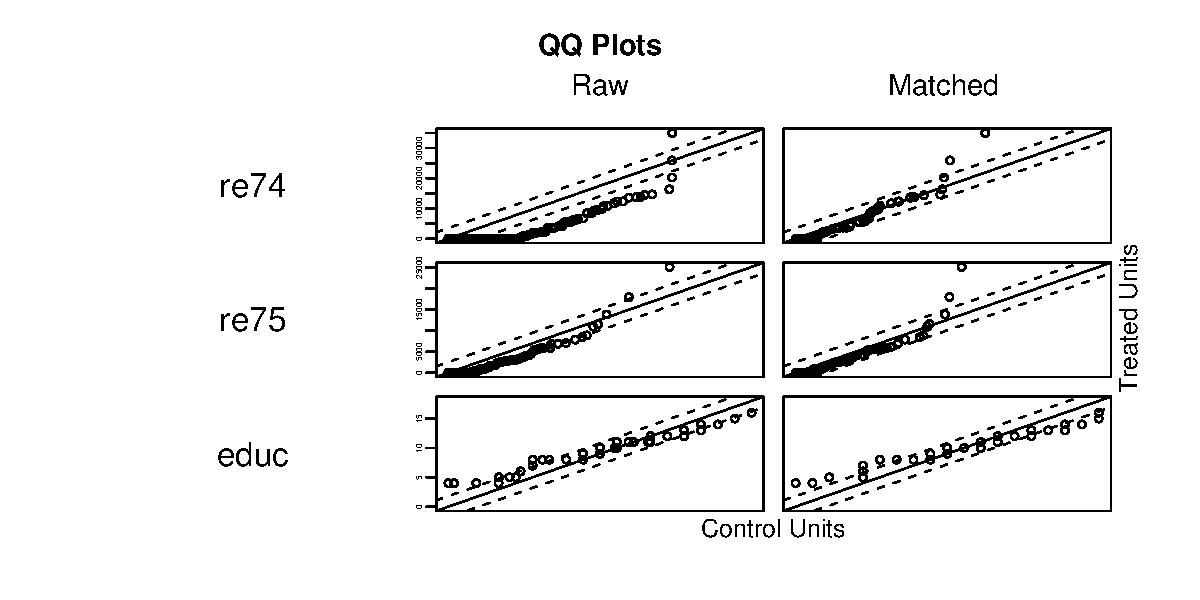
\includegraphics[scale=0.8]{figs/qqplotnn}}
    {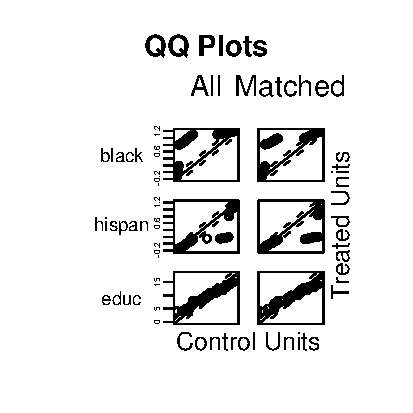
\includegraphics[scale=0.8]{figs/qqplotnn2}} \hfill
    \caption{Sample diagnostic QQ plots: Nearest Neighbor matching}
\label{diagqqnn}
\end{center}
\end{figure}

\begin{figure}[tbp]
  \begin{center}
%    \rotatebox{270}{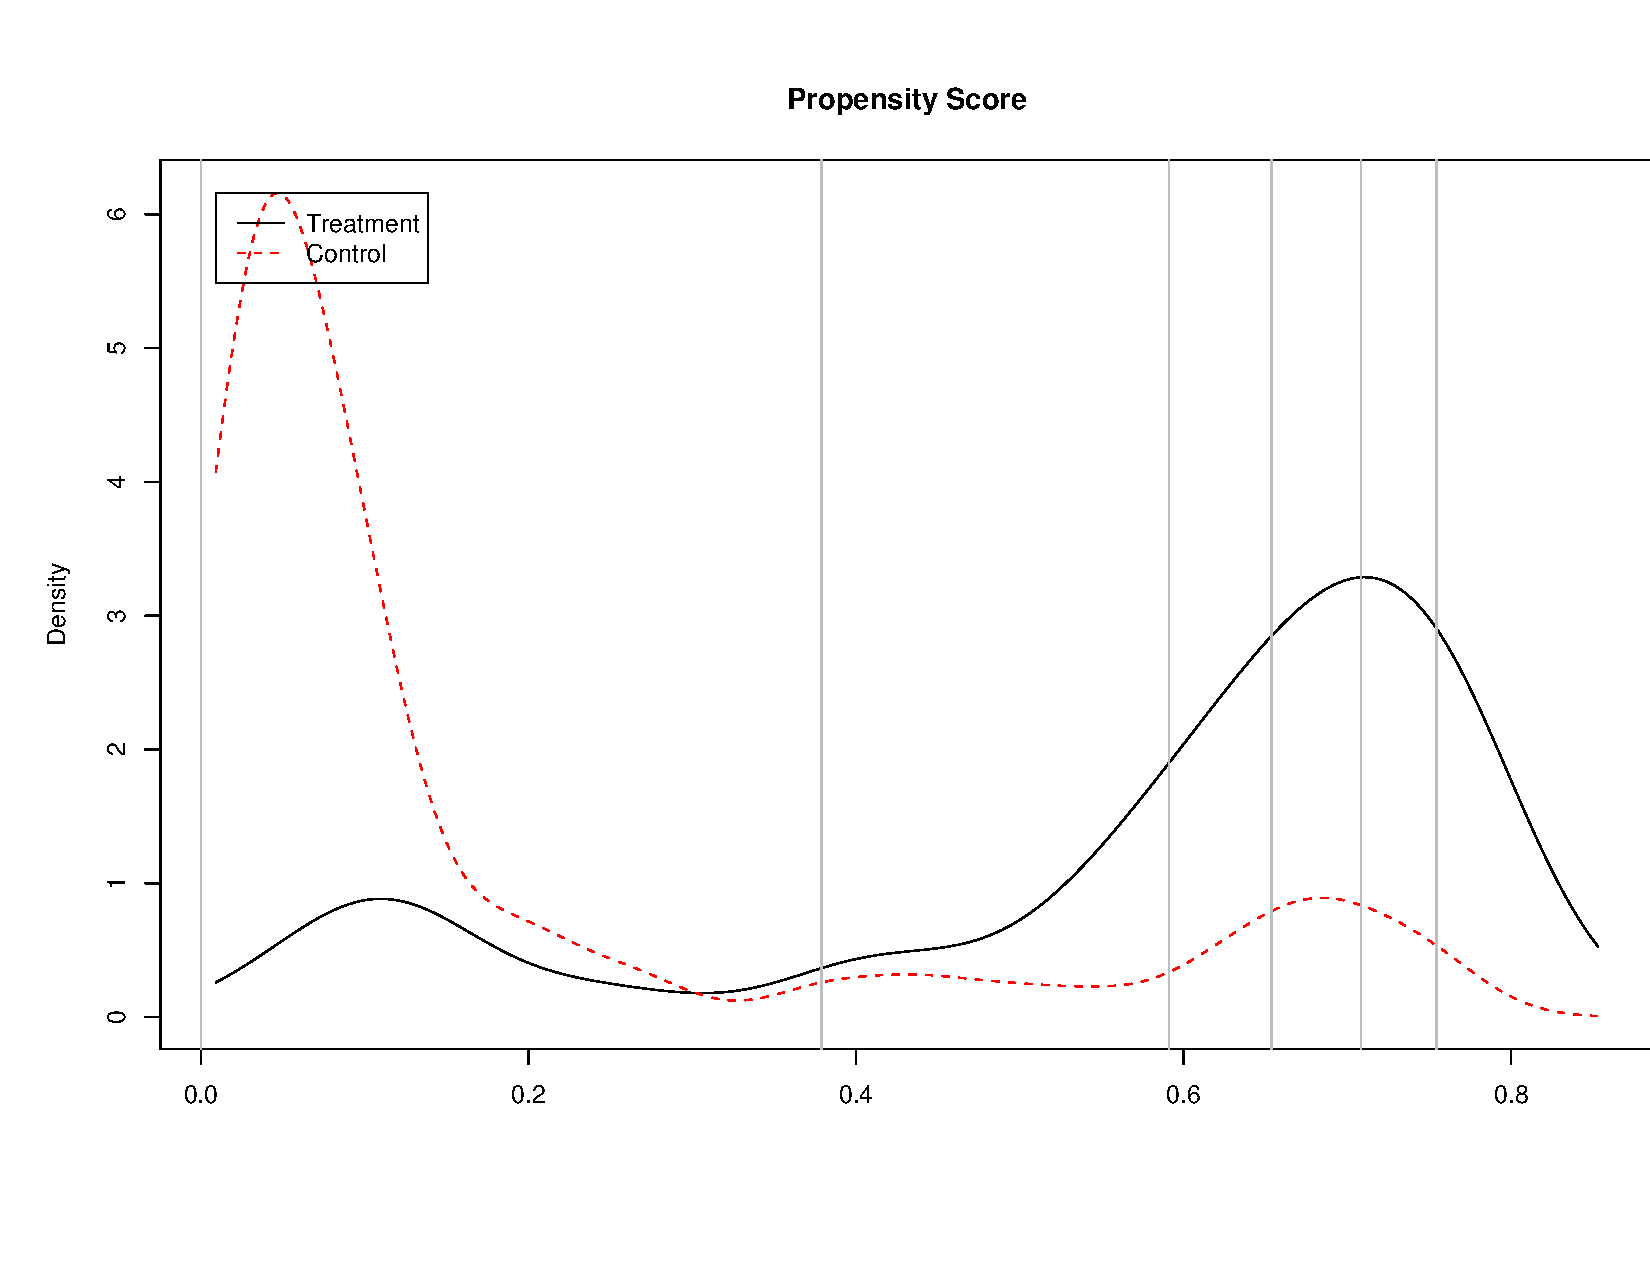
\includegraphics[height=2.85in,angle=0]{figs/subclass1}}
    {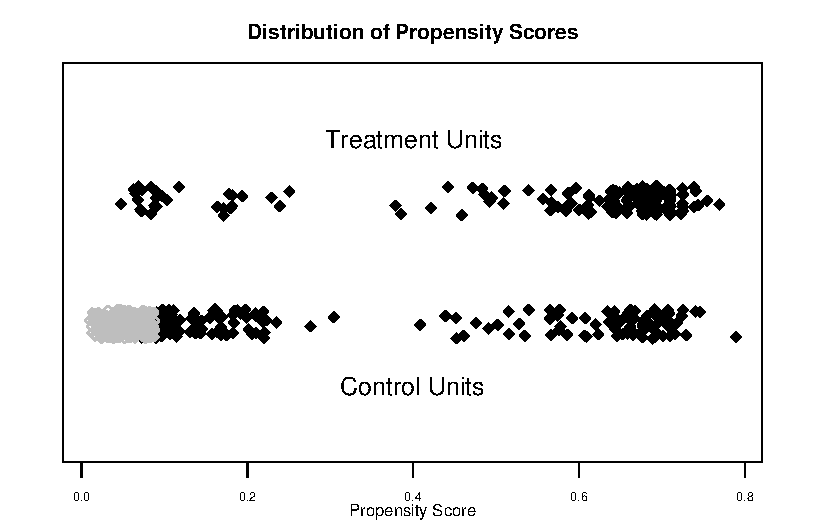
\includegraphics[scale=0.7]{figs/jitterplotnn}}
    \hfill
    \caption{Sample diagnostic jitter plot: Nearest Neighbor matching.
      Matched units shown in black, unmatched units shown in grey.}
\label{diagjitternn}
\end{center}
\end{figure}

The diagnostics are similar for subclassification, except that the
diagnostic statistics are printed out separately for each subclass,
and plots are generated separately for each subclass.

\begin{verbatim}

> m.outs <- matchit(treat ~ re74 + re75 + educ + black + hispan + age, data = lalonde, 
                    method = "subclass")
> print(summary(m.outs))

Call:
matchit(formula = treat ~ re74 + re75 + educ + black + hispan +     
        age, data = lalonde, method = "subclass", sub.by = "treat")

Summary of balance for all data:

         Means Treated Means Control Pooled SD   QQ Med  QQ Mean   QQ Max Std. Bias
distance      5.66e-01         0.187     0.284    0.732    0.535     0.84     1.792
re74          2.10e+03      5619.237  6477.964 3430.277 5155.851 13044.16    -0.721
re75          1.53e+03      2466.484  3295.679 1373.280 1511.706  9609.60    -0.290
educ          1.03e+01        10.235     2.628    1.414    0.962     5.66     0.055
black         8.43e-01         0.203     0.489    1.414    0.903     1.41     1.757
hispan        5.95e-02         0.142     0.322    0.000    0.119     1.41    -0.349
age           2.58e+01        28.030     9.881    1.414    4.650    14.14    -0.309
        
, , Subclass 1

         Means Treated Means Control Pooled SD    QQ Med   QQ Mean    QQ Max Std. Bias
distance      1.22e-01      7.62e-02  5.22e-02  5.48e-02  6.51e-02  1.23e-01  7.79e-01
re74          3.63e+03      6.33e+03  7.15e+03  4.59e+03  5.18e+03  1.30e+04 -3.38e-01
re75          2.23e+03      2.62e+03  3.30e+03  6.63e+02  1.15e+03  9.63e+03 -1.17e-01
educ          1.06e+01      1.03e+01  2.80e+00  1.41e+00  1.37e+00  9.90e+00  1.93e-01
black         6.45e-02      5.81e-03  1.03e-01  0.00e+00  4.56e-02  1.41e+00  2.35e-01
hispan        3.55e-01      1.77e-01  3.94e-01  0.00e+00  2.28e-01  1.41e+00  3.65e-01
age           2.50e+01      2.86e+01  1.05e+01  2.83e+00  6.56e+00  1.98e+01 -5.85e-01
        
, , Subclass 2

         Means Treated Means Control Pooled SD    QQ Med   QQ Mean    QQ Max Std. Bias
distance      5.39e-01      5.34e-01  6.46e-02  1.62e-02  1.99e-02  6.55e-02  6.29e-02
re74          7.53e+03      7.21e+03  5.92e+03  6.57e+02  1.23e+03  4.51e+03  5.56e-02
re75          4.11e+03      3.48e+03  5.01e+03  1.71e+03  2.12e+03  1.61e+04  1.10e-01
educ          9.00e+00      8.69e+00  3.47e+00  7.07e-01  1.29e+00  5.66e+00  1.03e-01
black         1.00e+00      1.00e+00  0.00e+00  0.00e+00  0.00e+00  0.00e+00          
hispan        0.00e+00      0.00e+00  0.00e+00  0.00e+00  0.00e+00  0.00e+00          
age           2.81e+01      3.33e+01  1.03e+01  9.33e+00  8.05e+00  1.98e+01 -6.36e-01
        
...
\end{verbatim}

\begin{comment}
, , Subclass 3

         Means Treated Means Control Pooled SD    QQ Med   QQ Mean    QQ Max Std. Bias
distance      6.46e-01      6.45e-01  1.16e-02  1.32e-03  2.86e-03  1.30e-02  7.54e-02
re74          8.92e+02      1.40e+03  1.82e+03  5.43e+02  8.26e+02  2.12e+03 -3.15e-01
re75          7.07e+02      1.46e+03  2.19e+03  2.91e+02  9.44e+02  8.97e+03 -5.02e-01
educ          8.93e+00      9.12e+00  1.32e+00  0.00e+00  4.37e-01  2.83e+00 -1.57e-01
black         1.00e+00      1.00e+00  0.00e+00  0.00e+00  0.00e+00  0.00e+00          
hispan        0.00e+00      0.00e+00  0.00e+00  0.00e+00  0.00e+00  0.00e+00          
age           2.39e+01      1.96e+01  7.08e+00  3.80e+00  6.26e+00  2.00e+01  5.47e-01
        
, , Subclass 4

         Means Treated Means Control Pooled SD    QQ Med   QQ Mean    QQ Max Std. Bias
distance      6.77e-01      6.78e-01  8.23e-03  4.31e-03  4.32e-03  1.19e-02 -7.99e-02
re74          3.90e+02      7.11e+02  8.22e+02  0.00e+00  4.42e+02  1.68e+03 -4.35e-01
re75          1.19e+03      6.84e+02  1.47e+03  1.52e+02  7.70e+02  3.23e+03  3.06e-01
educ          1.00e+01      1.06e+01  9.21e-01  1.41e+00  8.08e-01  2.83e+00 -7.38e-01
black         1.00e+00      1.00e+00  0.00e+00  0.00e+00  0.00e+00  0.00e+00          
hispan        0.00e+00      0.00e+00  0.00e+00  0.00e+00  0.00e+00  0.00e+00          
age           2.35e+01      2.22e+01  7.99e+00  2.83e+00  4.48e+00  1.13e+01  1.95e-01
        
, , Subclass 5

         Means Treated Means Control Pooled SD    QQ Med   QQ Mean    QQ Max Std. Bias
distance      6.94e-01      6.97e-01  3.20e-03  1.09e-03  3.37e-03  1.07e-02 -9.86e-01
re74          9.41e+01      3.26e+02  4.43e+02  0.00e+00  1.58e+02  8.01e+02 -6.03e-01
re75          4.05e+02      3.08e+02  1.23e+03  0.00e+00  1.27e+03  7.78e+03  7.26e-02
educ          1.10e+01      1.14e+01  4.28e-01  0.00e+00  6.06e-01  1.41e+00 -1.66e+00
black         1.00e+00      1.00e+00  0.00e+00  0.00e+00  0.00e+00  0.00e+00          
hispan        0.00e+00      0.00e+00  0.00e+00  0.00e+00  0.00e+00  0.00e+00          
age           2.67e+01      2.23e+01  6.11e+00  9.90e+00  6.87e+00  1.27e+01  8.19e-01        
\end{comment}
\begin{verbatim}
, , Subclass 6

         Means Treated Means Control Pooled SD    QQ Med   QQ Mean    QQ Max Std. Bias
distance      7.20e-01      7.24e-01  1.81e-02  2.63e-03  5.47e-03  2.88e-02 -2.90e-01
re74          0.00e+00      2.70e+02  3.97e+02  0.00e+00  3.82e+02  3.63e+03      -Inf
re75          5.19e+02      1.66e+03  2.34e+03  0.00e+00  1.33e+03  6.83e+03 -6.96e-01
educ          1.25e+01      1.26e+01  1.20e+00  0.00e+00  2.33e-01  1.41e+00 -1.35e-01
black         1.00e+00      1.00e+00  0.00e+00  0.00e+00  0.00e+00  0.00e+00          
hispan        0.00e+00      0.00e+00  0.00e+00  0.00e+00  0.00e+00  0.00e+00          
age           2.76e+01      2.70e+01  7.84e+00  2.45e+00  3.32e+00  1.13e+01  8.69e-02
        
Sample sizes by subclasses:

        Subclass 1 Subclass 2 Subclass 3 Subclass 4 Subclass 5 Subclass 6
Treated         31         31         30         31         31         31
Control        344         26         17         21          7         14
Total          375         57         47         52         38         45

Summary of balance across subclasses

         Means Treated Means Control Pooled SD   QQ Med  QQ Mean   QQ Max Std. Bias
distance      5.66e-01      5.59e-01  1.44e-02   0.0135 1.69e-02 4.23e-02   -0.0741
re74          2.10e+03      2.72e+03  1.59e+03 967.1902 1.37e+03 4.30e+03      -Inf
re75          1.53e+03      1.71e+03  1.18e+03 470.4902 1.26e+03 8.75e+03   -0.1360
educ          1.03e+01      1.05e+01  8.20e-01   0.5924 7.93e-01 4.01e+00   -0.4002
black         8.43e-01      8.33e-01  1.72e-02   0.0000 7.64e-03 2.37e-01       NaN
hispan        5.95e-02      2.97e-02  6.61e-02   0.0000 3.82e-02 2.37e-01       NaN
age           2.58e+01      2.55e+01  3.46e+00   5.1973 5.92e+00 1.58e+01    0.0687
        
Percent Balance Improvement:

         Mean QQ Med QQ Mean QQ Max Std. Bias
distance 98.1   98.2    96.8  94.97      95.9
re74     82.4   71.8    73.4  67.05      -Inf
re75     81.4   65.7    16.3   8.94      53.1
educ     -3.3   58.1    17.6  29.05    -628.1
black    98.5  100.0    99.2  83.24       NaN
hispan   64.0    0.0    67.8  83.24       NaN
age      86.8 -267.5   -27.3 -11.72      77.8

\end{verbatim}
Similarly, we can examine the balance within each subclass graphically:
\begin{verbatim}
> plot(m.outs)
> plot(m.outs, type="jitter")
\end{verbatim}    

\begin{figure}[tbp]
  \begin{center}
%    \rotatebox{270}{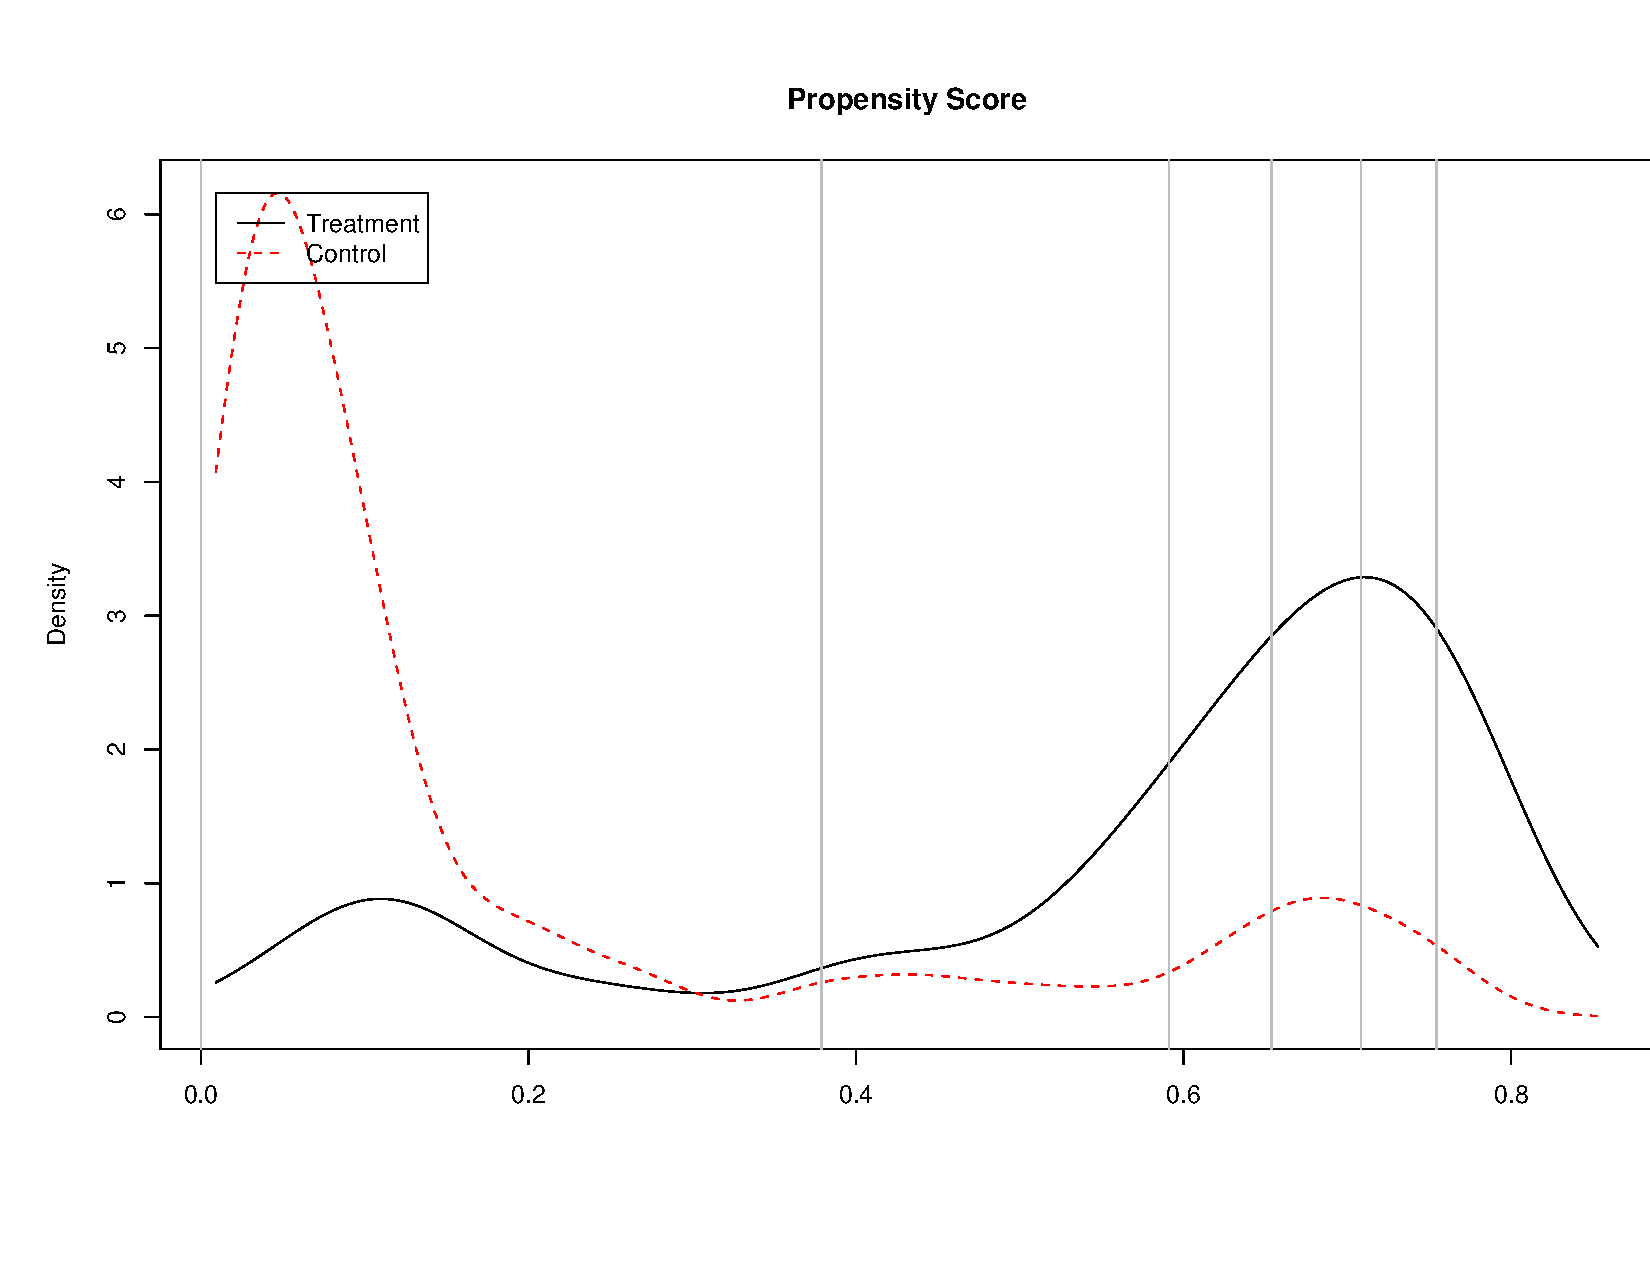
\includegraphics[height=2.85in,angle=0]{figs/subclass1}}
    {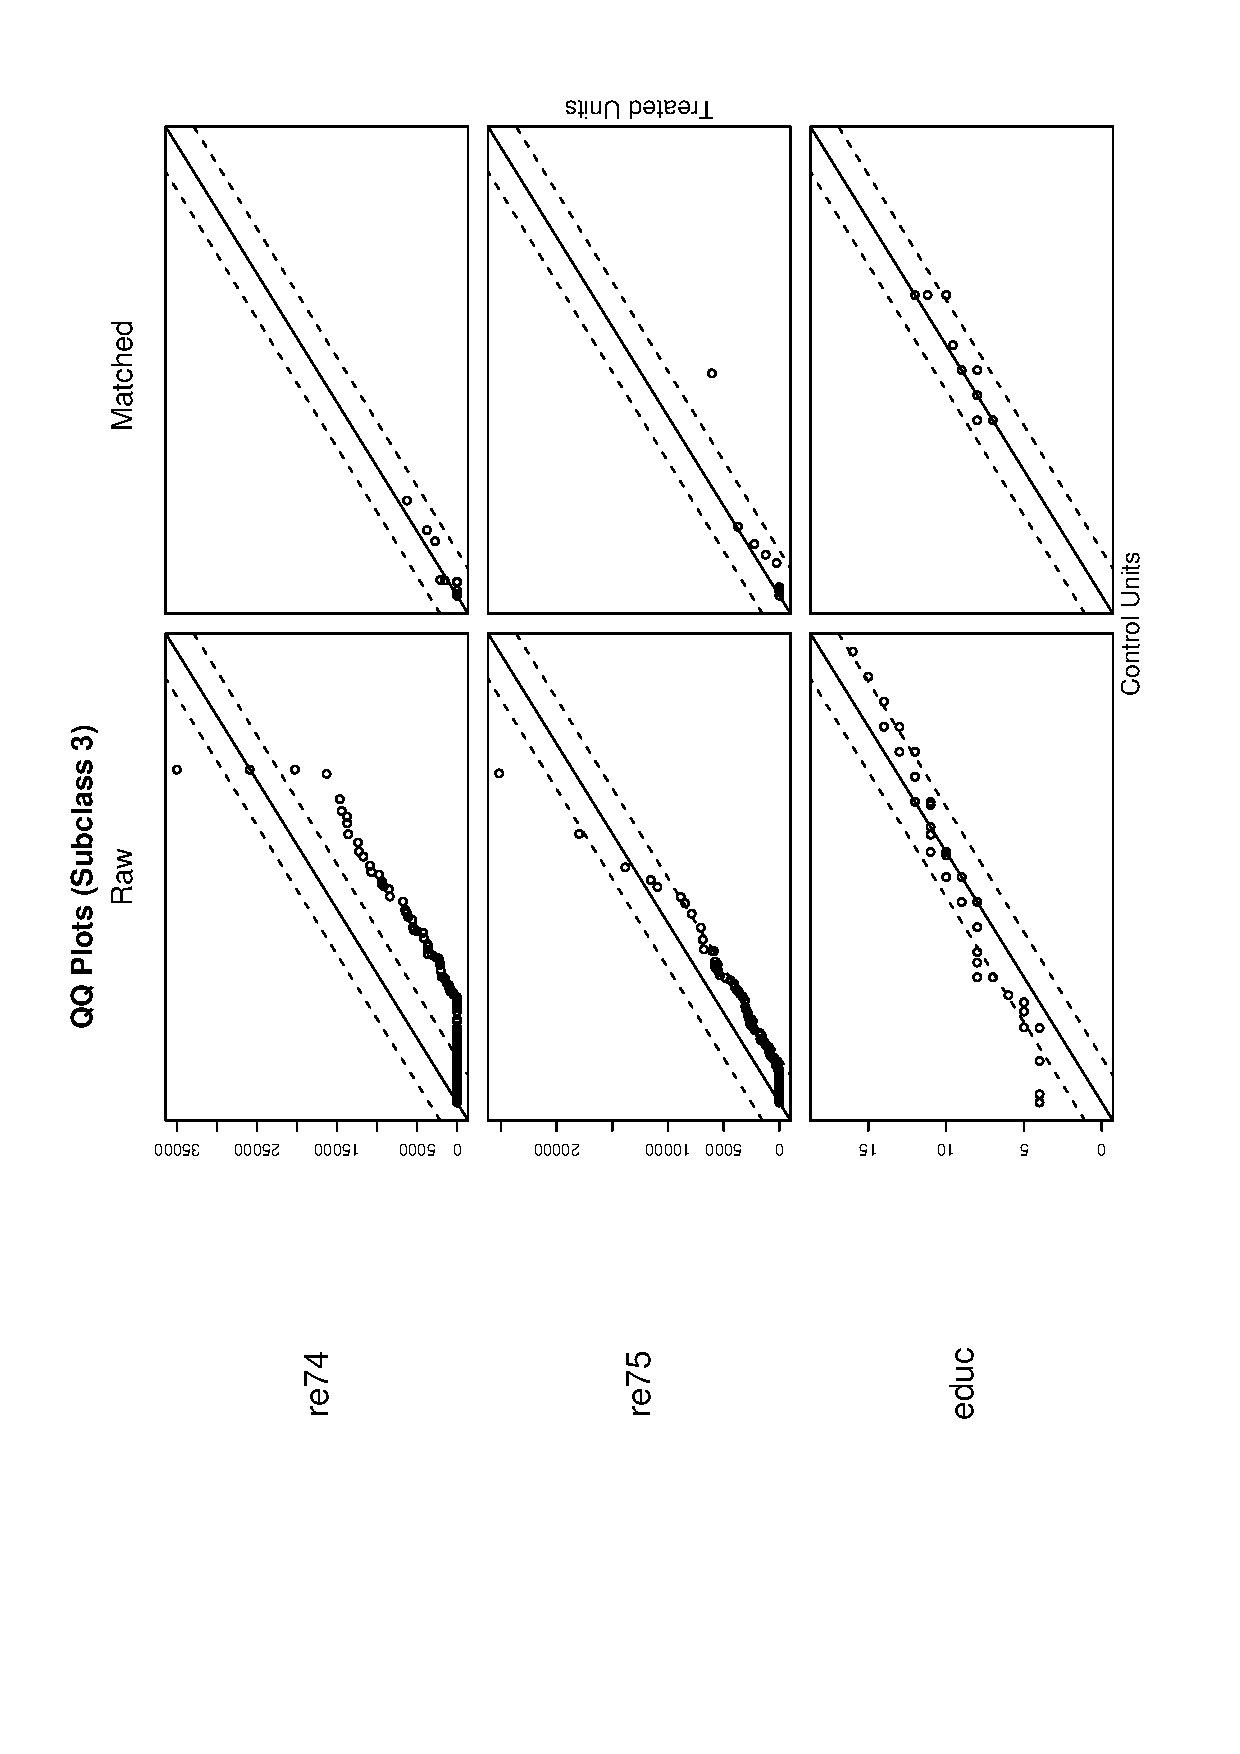
\includegraphics[scale=.8]{figs/qqplotsub}}
    {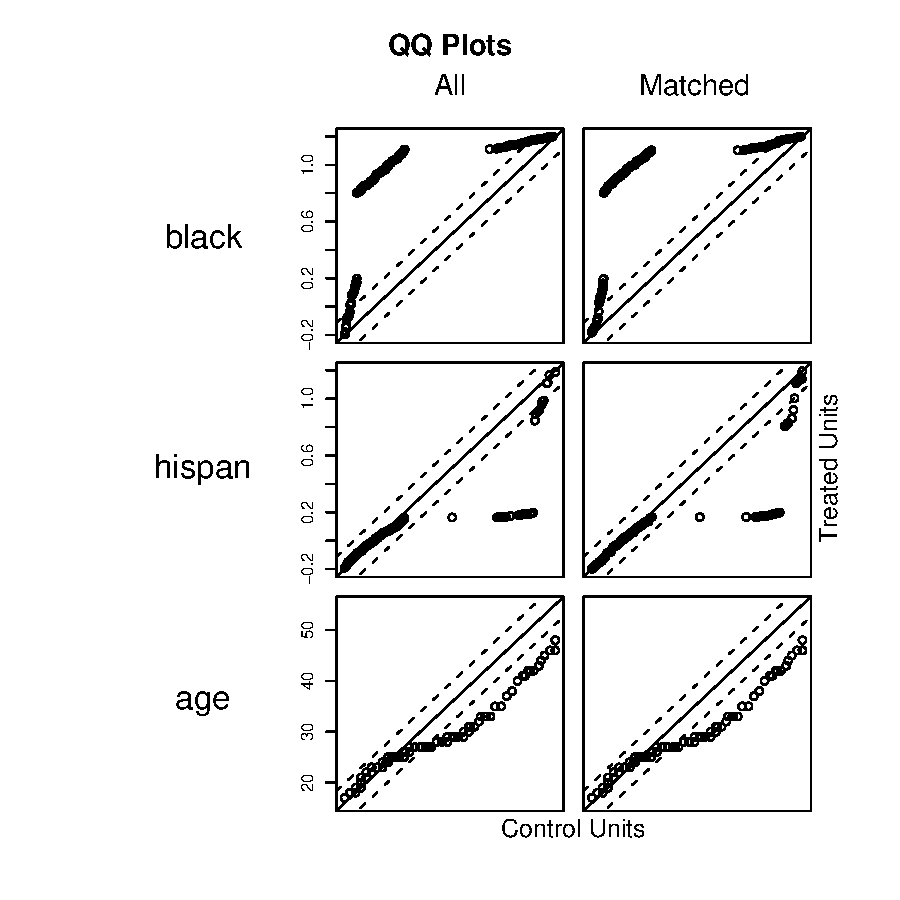
\includegraphics[scale=.8]{figs/qqplotsub2}}
    \hfill
    \caption{Sample diagnostic QQ plots: Subclassification}
\label{diagqqsub}
\end{center}
\end{figure}

\begin{figure}[tbp]
  \begin{center}
%    \rotatebox{270}{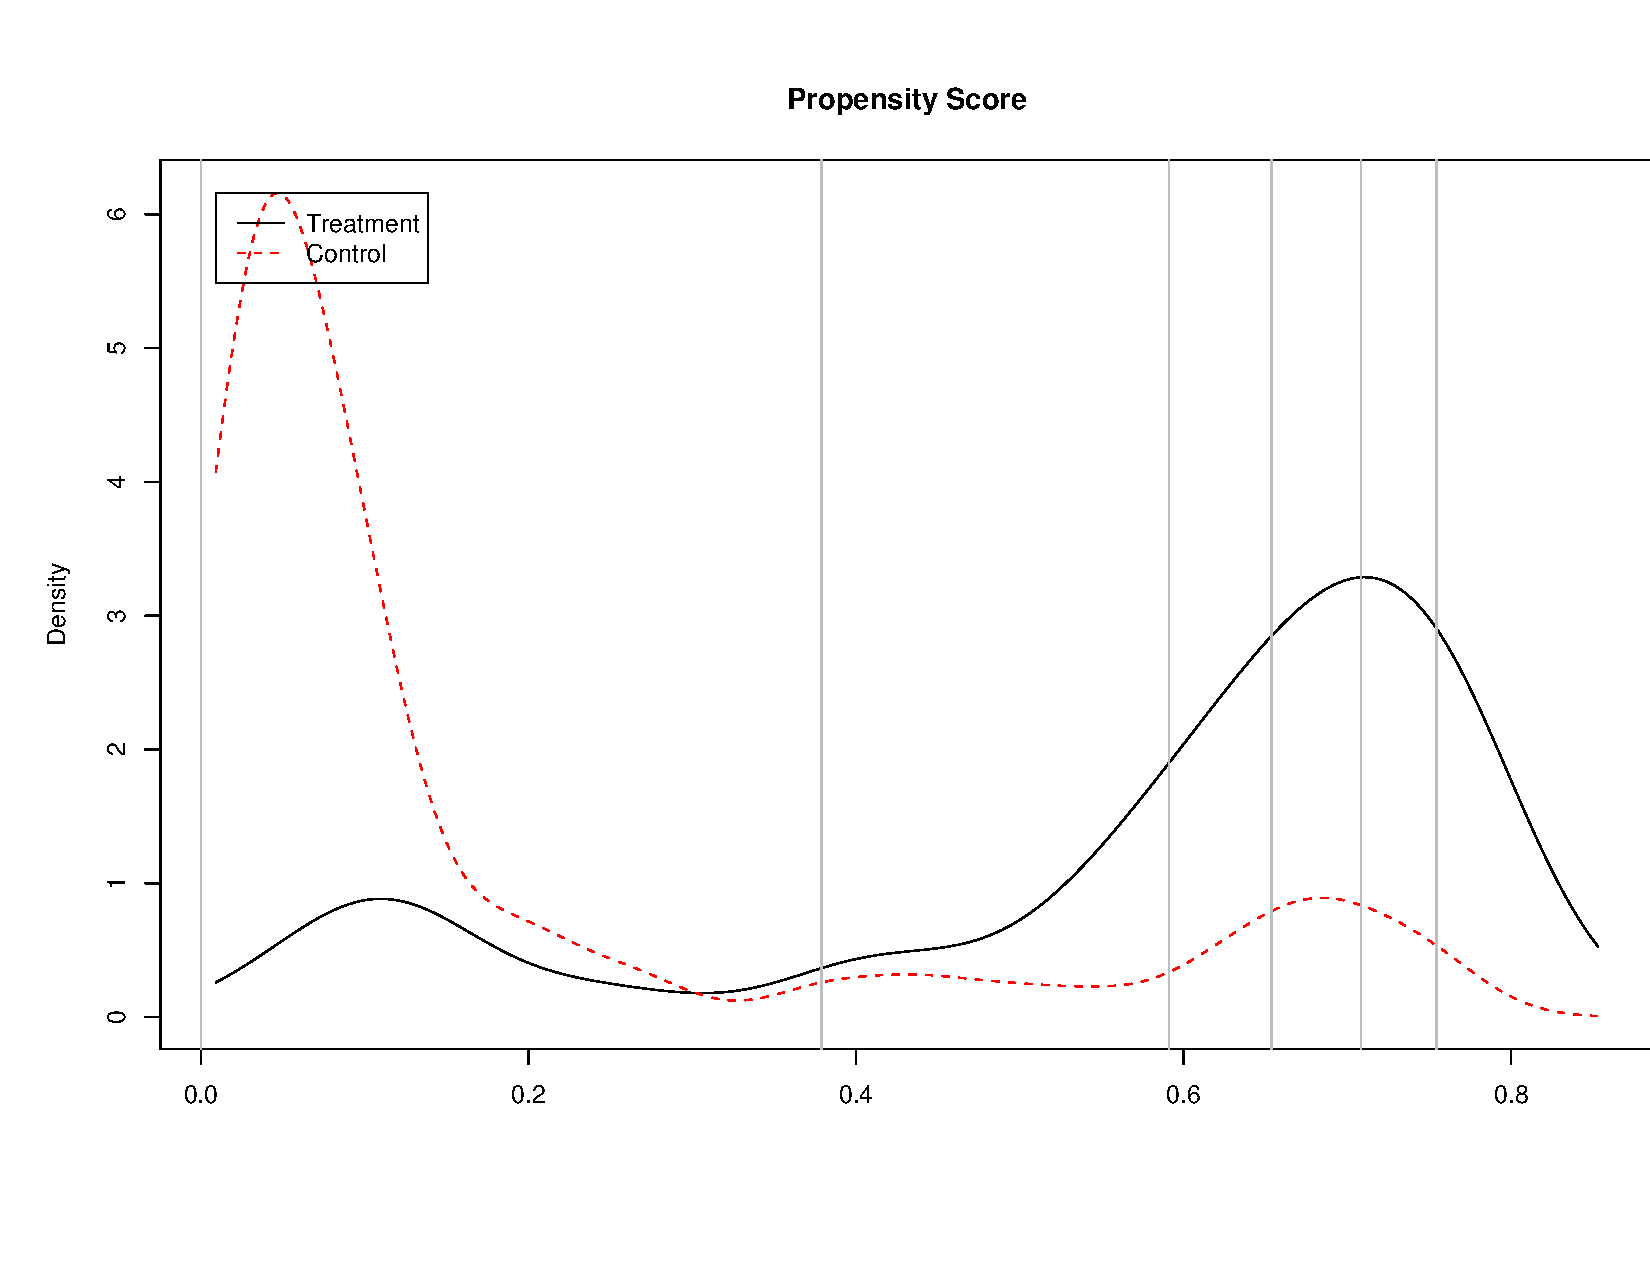
\includegraphics[scale=0.5,angle=0]{figs/subclass1}}
    {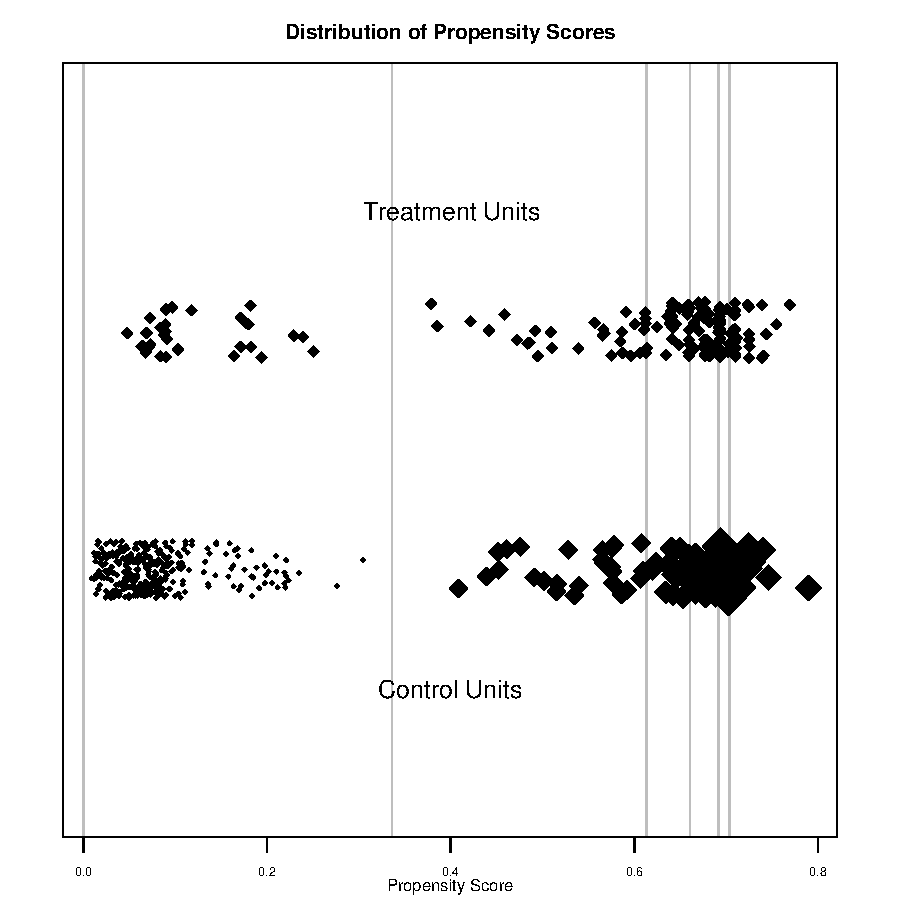
\includegraphics[scale=0.7]{figs/jitterplotsub}}
    \hfill
    \caption{Sample diagnostic jitter plot: Subclassification.  Vertical lines indicate the subclass cut points.}
\label{diagjittersub}
\end{center}
\end{figure}
Further examples of the summary statistics and diagnostic plots can be
seen in the demos for each of the specific matching methods (see
Section \ref{methods}).

\subsubsection{{\tt match.data()}}
\label{subsec:match.data}

After matching, one might wish to obtain the matched data set for
subsequent analyses (see Section~\ref{sec:analysis}) and other
purposes. We provide the function {\tt match.data()} to allow users to
obtain the matched data set.
\begin{verbatim}
m.data <- match.data(object, group = "all", distance = "distance", weights = "weights",
                     subclass = "subclass")
\end{verbatim}
The output of the function {\tt match.data()} is the original data
frame where additional information about matching (i.e., distance
measure as well as resulting weights and subclasses) is added,
restricted to units that were matched.

\paragraph{Inputs}

{\tt match.data()} takes the following inputs:
\begin{enumerate}
\item {\tt object} is the output object from {\tt matchit()}. This is
  a required input.
\item {\tt group} specifies for which matched group the user wants to
  extract the data. Available options are {\tt "all"} (all matched
  units), {\tt "treat"} (matched units in the treatment group), and
  {\tt "control"} (matched units in the control group). The default is
  {\tt "all"}.
\item {\tt distance} specifies the variable name used to store the
  distance measure. The default is {\tt "distance"}.
\item {\tt weights} specifies the variable name used to store the
  resulting weights from matching. The default is {\tt "weights"}. See
  Section~\ref{subsec:weights} for more details on the weights.
\item {\tt subclass} specifies the variable name used to store the
  subclass indicator. The default is {\tt "subclass"}.
\end{enumerate}

\paragraph{Examples}

Here, we present examples for using {\tt match.data()}. Users can run
these commands by typing {\tt demo(match.data)} at the R prompt.
\begin{verbatim}
## load the Lalonde data
data(lalonde)

## run a nearest neighbor matching
m.out1 <- matchit(treat ~ re74 + re75 + age + educ, data = lalonde, method = "nearest",  
                  distance = "logit")

## obtain matched data 
m.data1 <- match.data(m.out1)

## summarize the resulting matched data
summary(m.data1)

## obtain matched data for the treatment group
m.data2 <- match.data(m.out1, group = "treat")
summary(m.data2)

## obtain matched data for the control group
m.data3 <- match.data(m.out1, group = "control")
summary(m.data3)

## run a subclassification method
m.out2 <- matchit(treat ~ re74 + re75 + age + educ, data=lalonde, method = "subclass")

## specify different names
m.data4 <- match.data(m.out2, subclass = "block", weights = "w",
                      distance = "pscore")
## print the variable names of the matched data
names(m.data4)
\end{verbatim}




%%%%%%%%%%%%%%%%%%%%%%%%%%%%%%%%%%%%%%%%%%%%%%%%%%%%%%%%%%%%%%%%%%%%%%%%%

\section{What's New?}

\begin{itemize}
\item \textbf{2.0-1} (??, 2005): Stable release for R 2.1. Major revisions.
\item \textbf{1.0-1} (January 3, 2005): Stable release for R 2.0. The
  first official version of \MatchIt
\end{itemize}


%%%%%%%%%%%%%%%%%%%%%%%%%%%%%%%%%%%%%%%%%%%%%%%%%%%%%%%%%%%%%%%%%%%%%%%%%


\section{Frequently Asked Questions}

\subsection{Can I use a Difference-in-Difference Estimator for Matched
  Data?}

A difference-in-differences (DID) analysis can be easily conducted
with \MatchIt.  If we were interested in the DID matching estimate in
the Lalonde data, we could simply include {\texttt re75} as a
covariate in the preprocessing step.  Then the analysis can be
performed on the change in income from 1975 to 1978: {\tt re78}-{\tt
  re75}.  Time-varying covariates (of which none exist in the Lalonde
data) should of course also be differenced for the DID estimator.

\subsection{How Exactly are the Weights Created?}
\label{subsec:weights}

Each type of matching method can be thought of as creating groups of
units with at least one treated unit and at least one control unit in
each group.  In exact matching, subclassification, or full matching,
these groups are the subclasses formed, and the number of treated and
control units will vary quite a bit across subclasses.  In nearest
neighbor or optimal matching, thee groups are the pairs (or sets) of
treated and control units matched: in 1:1 nearest neighbor matching
there will be one treated unit and one control unit in each group.  In
2:1 nearest neighbor matching there will be one treated unit and two
control units in each group.  Unmatched units receive a weight of 0.
All matched treated units receive a weight of 1.

The weights for matched control units are formed as follows:
\begin{enumerate}
\item Within each group, each control unit is given a preliminary
  weight of $n_{ti}/n_{ci}$, where $n_{ti}$ and $n_{ci}$ are the
  number of treated and control units in group $i$, respectively.
\item If matching is done with replacement, each control unit's weight
  is added up across the groups in which it was matched.
\item The control group weights are scaled to sum to the number of
  uniquely matched control units.
\end{enumerate}

With subclassification, when the analysis is done separately within
each subclass and then aggregated up across the subclasses, these
weights will generally not be used, but they may be used for full
matching or nearest neighbor matching if the number of control units
matched to each treated unit varies.

\subsection{How Do I Create Observation Names?}
\label{rnames}

Since the diagnostics often make use of the observation names of the
data frame, you may find it helpful to specify observation names for
the data input.  Use the \texttt{row.names} command to achieve this.
For example, to assign the names ``Dan'', ``Kosuke'', ``Liz'' and
``Gary'' to a data frame with the first four observations in the
Lalonde data, type:

\begin{verbatim}
> test <- lalonde[1:4,]  #taking a lalonde subset
> row.names(test) <- c("Dan","Kosuke","Liz","Gary")  #assigning row names
> print(test)
       treat age educ black hispan married nodegree re74 re75      re78
Dan        1  37   11     1      0       1        1    0    0  9930.046
Kosuke     1  22    9     0      1       0        1    0    0  3595.894
Liz        1  30   12     1      0       0        0    0    0 24909.450
Gary       1  27   11     1      0       0        1    0    0  7506.146
\end{verbatim} 


\subsection{How Do I Ensure Replicability As \MatchIt\ Versions Develop?}

As the literature on matching techniques is rapidly evolving,
\MatchIt\ will strive to incorporate new developments. \MatchIt\ is
thereby an evolving program.  Users may be concerned that analysis
written in a particular version may not be compatible with newer
versions of the program.  The primary way to ensure that replication
archives remain valid is to record the version of \MatchIt\ that was
used in the analysis.  Our website maintains binaries of all public
release versions, so that researchers can replicate results exactly
with the appropriate version (for Unix-based platforms, see
\hlink{http://gking.harvard.edu/src/contrib/}{http://gking.harvard.edu/src/contrib/};
for windows, see
\hlink{http://gking.harvard.edu/bin/windows/contrib/}{http://gking.harvard.edu/bin/windows/contrib/}).

In addition, users may find it helpful to install packages with
version control, using the {\tt installWithVers} command with {\tt
  install.packages}.  So for example, in the windows R console, users
may download the appropriate version from our website and install the
package with version control by:

\begin{verbatim}
install.packages(choose.files('',filters=Filters[c('zip','All'),]),
                 .libPaths()[1],installWithVers=T,CRAN=NULL)
\end{verbatim}

R CMD INSTALL similarly permits users to specify this version using
the {\tt --with-package-versions} option.  After having specified
version control, different versions of the program may be called as
necessary.  Similar advice may also be appropriate for version control
for R more generally.

\subsection{What Do I Do about Missing Data?}

\MatchIt\ requires complete data sets, with no missing values (other
than potential outcomes of course).  If there are missing values in
the data set, imputation techniques should be used first to fill in
(``impute'') the missing values (both covariates and outcomes), or the
analysis should be done using only complete cases (which we do not in
general recommend).  For imputation software, see Amelia at
(\hlink{http://gking.harvard.edu/stats.shtml}{http://gking.harvard.edu/stats.shtml})
or other programs at
\hlink{http://www.multiple-imputation.com}{http://www.multiple-imputation.com}.
For more information on missing data and imputation methods, see
\cite{KinHonJos01}.

\subsection{Why Preprocessing?}

The purpose of matching is to approximate an experimental template,
where the matching procedure approximates random assignment of
treatment in order to balance covariates between treatment and control
groups.  Separation of the estimation procedure into two steps
simulates the research design of an experiment, where no information
on outcomes is known at the point of experimental design and
randomization.  Much like an experimenter cannot easily rerun an
experiment if the outcome was not satisfactory, the separation of the
balancing process in \MatchIt\ from the analysis process afterwords
helps keep clear the goal of balancing control and treatment groups
and makes it less likely that the user will inadvertently cook the
books in his or her favor.


% see gkbibtex/cvstricks.tex
\clearpage
\bibliographystyle{polisci}
\bibliography{gk,gkpubs}

\end{document}

